\documentclass[11pt,a4paper]{article}

% --- packages ---------------------------------------------------------
\usepackage[utf8]{inputenc}
\usepackage[T1]{fontenc}
\usepackage[margin=1in]{geometry}
\usepackage{amsmath,amssymb,amsthm}
\usepackage{bm}
\usepackage{mathtools}
\usepackage{booktabs}
\usepackage{array}
\usepackage{xcolor}
\usepackage{graphicx}
\usepackage{float}
\usepackage{caption}
\usepackage{subcaption}
\usepackage{enumitem}
\usepackage{microtype}
\usepackage{hyperref}
\hypersetup{colorlinks=true,
            linkcolor=blue!50!black,
            citecolor=blue!50!black,
            urlcolor=blue!50!black,
            pdftitle={Cascaded chi3 in a lithium niobate microring}}

% --- macros (consistent with the metasurface note) --------------------
\newcommand{\eps}{\varepsilon}
\newcommand{\bvec}[1]{\mathbf{#1}}
\newcommand{\f}{\bvec{f}}
\newcommand{\chitwo}{\chi^{(2)}}
\newcommand{\chithree}{\chi^{(3)}}
\newcommand{\Dom}{\Delta\omega}
\newcommand{\Ucasc}{U_{\text{casc}}}
\newcommand{\Unat}{U_{\text{nat}}}
\newcommand{\kcasc}{\kappa_{\text{casc}}}
\newcommand{\Veff}{V_{\text{eff}}}
\newcommand{\Aeff}{A_{\text{eff}}}
\newcommand{\etanorm}{\eta_{\text{SHG}}}

\captionsetup{labelfont={small,bf}, font=small, labelsep=period}
\graphicspath{{cascaded_chi3/figures/ring/}{cascaded_chi3/figures/}}

\setlength{\parskip}{0.4em}

% =======================================================================
\begin{document}

\title{Cascaded \texorpdfstring{$\chi^{(2)}{:}\chi^{(2)}\to\chi^{(3)}_{\text{eff}}$}{chi2:chi2 -> chi3eff}
       in a Doubly-Resonant Lithium Niobate Microring\\[4pt]
       \large Feasibility, observables, and comparison with a native-\texorpdfstring{$\chi^{(3)}$}{chi3} ring}
\author{}
\date{\today}
\maketitle

\begin{abstract}
\noindent
We adapt the cascaded $\chi^{(2)}{:}\chi^{(2)}$ Kerr analysis of the
metasurface note to a travelling-wave thin-film lithium niobate (LN)
microring with loaded $Q_1\sim10^5$--$10^6$ at the fundamental.  Three
things change qualitatively relative to the metasurface, and all three
work in the microring's favour.  First, the absolute scale of the
cascade is no longer a modelling unknown: the $\chi^{(2)}$
photon--photon coupling rate $g$ is fixed by the \emph{measured}
normalised second-harmonic (SH) generation efficiency through a relation
we derive and check against the published expression, so the
$O(1)$ ``bridge'' constant that limited the metasurface sample analysis
disappears.  Second, because $\omega_2=2\omega_1$ while $Q_2\lesssim Q_1$,
the SH mode is intrinsically \emph{broader} than the fundamental, so the
cascade costs no device bandwidth --- the opposite of the metasurface,
where the SH linewidth was the bottleneck.  Third, loaded $Q_2\sim3\times10^5$ at
$780$~nm is experimentally plausible with precedent, rather than
exceptional.  Taking the demonstrated PPLN microring coupling
$g/2\pi=1.2$~MHz and scaling it to a smaller target ring
($g/2\pi\simeq1.4$~MHz, an extrapolation), the cascaded Kerr coefficient
exceeds the native LN Kerr by $R\simeq1.8\times10^{3}$ at the
conservative operating point $\Dom=2\gamma_2$, equivalent to
$n_2^{\text{eff}}\simeq-3.3\times10^{-16}$ m$^2$/W.  Bistability moves
from $14$~mW to $32$--$37\,\mu$W; a multimode Bogoliubov stability
calculation puts the parametric threshold at $8.4\,\mu$W against
$9.4$~mW natively.  Without periodic poling the advantage collapses to
$R\simeq13$, so poling is the enabling step.  Two design rules follow:
bistability and single-pair parametric gain both require the
\emph{pump-frame} mismatch to satisfy
$|\Delta_{\text{eff}}|>\tfrac{\sqrt3}{2}\gamma_2$, where
$\Delta_{\text{eff}}=\Dom-2\delta_1$; and the Kerr description requires
the envelope bandwidth to stay below $\sqrt{\kappa_2^2+\delta_2^2}$,
which for this device is $27\kappa_1$.  The binding obstacles are
thermal and photorefractive shifts, which are within a factor of two of
the cascaded Kerr at the relevant powers.  The cascade is \emph{odd} in
$\Dom$ where they are, to leading order, \emph{even}, and lithium
niobate's own Pockels effect tunes $\Dom$ by $2.4\gamma_2$ per
V/$\mu$m, so an electro-optically dithered, antisymmetric-in-$\Dom$
lock-in measurement suppresses them.  That measurement is the
recommended first experiment.  The cascade is \emph{not} a route to
single-photon anharmonicity: the dispersive figure of merit is
$\sim(g/\kappa_1)(g/\kappa_2)$, quadratically worse than the resonant
$g/\kappa_1$.
\end{abstract}

\tableofcontents

% =======================================================================
\section{Setting and goal}\label{sec:setting}

The main note derives the cascaded response
$\chithree_{\text{casc}}(\omega_1)$ of a doubly-resonant dielectric
metasurface: a quasi-BIC at $\omega_1$ and a high-$Q$ mode near
$2\omega_1$, with the SH adiabatically eliminated to leave a Kerr-like
term on the fundamental.  The same two-mode structure describes a
doubly-resonant $\chitwo$ microring, and the derivation carries over
essentially unchanged.  What changes is the \emph{numbers}, and they
change by three orders of magnitude.

The reason is structural.  The metasurface enhancement was
$R\propto Q_2$ with $Q_2\sim4\times10^3$ realistically available in a
quasi-BIC; the four fabricated SH-only samples and Design~6 delivered
$R^{(1\mathrm R)}=0.4$--$2.5$ once the true modal overlaps were measured.
A thin-film LN microring routinely reaches $Q_2\sim3$--$6\times10^5$ at
the SH wavelength, two orders of magnitude higher, and the modal overlap
problem is solved by a different mechanism --- quasi-phase matching via
periodic poling, which recovers the full $d_{33}$ over the entire
circumference.

Three questions organise what follows.

\begin{enumerate}[label=(\roman*),leftmargin=2em]
\item \textbf{Is the platform good enough?}  Section~\ref{sec:R}
  answers this with the enhancement ratio $R$, anchored on a measured
  device rather than on an assumed overlap.
\item \textbf{Which observables can be demonstrated, and how do they
  compare with the same ring running on its native $\chithree$?}
  Section~\ref{sec:observables} works through sign-tunability,
  bistability, switching, cross-phase modulation, parametric
  oscillation, and single-photon anharmonicity.
\item \textbf{What stops it?}  Section~\ref{sec:competing} quantifies
  thermal and photorefractive shifts, which are the real competition,
  and Section~\ref{sec:experiment} turns the answer into a measurement
  protocol.
\end{enumerate}

\paragraph{Relation to prior work.}  Cascaded quadratic nonlinearity in
$\chitwo$ microresonators is not new: it is the accepted mechanism
behind ``quadratic'' frequency combs in thin-film LN
microresonators~\cite{QuadraticComb2024}, and resonantly coupled
$\chitwo$ microrings have been pushed toward single-photon
anharmonicity~\cite{Lu2020,Lu2019}, in the lineage of the bulk cascading
literature~\cite{DeSalvo1992,Stegeman1996,Khurgin1997}.  What is new here is the
systematic, observable-by-observable comparison against the
\emph{native} $\chithree$ of the same ring at matched operating points,
the three design rules of Section~\ref{sec:rules}, and the
antisymmetric-in-$\Dom$ protocol that separates the cascade from thermal
and photorefractive backgrounds.

% =======================================================================
\section{Conventions and the map to the metasurface note}\label{sec:conv}

\paragraph{Photon-number convention.}  For the ring it is cleanest to
work in the Hamiltonian (photon-number) convention standard in the
$\chitwo$ microresonator literature.  With $a$ the fundamental (FM) mode
at $\omega_1$ and $b$ the SH mode at $\omega_2\approx2\omega_1$,
\begin{equation}
  \hat H/\hbar=\omega_1 a^\dagger a+\omega_2 b^\dagger b
               +g\bigl[(a^\dagger)^2 b+a^2 b^\dagger\bigr],
  \label{eq:H}
\end{equation}
which is Eq.~(1) of Ref.~\cite{Lu2020}.  Here $g$ is the vacuum
photon--photon coupling rate, in rad/s.

\paragraph{Loss rates: two conventions, one factor of two.}  The
microresonator literature uses the HWHM \emph{amplitude} decay rate
$\kappa_n=\omega_n/(2Q_n)$; the metasurface note uses the \emph{energy}
decay rate $\gamma_n=\omega_n/Q_n$, which is the FWHM linewidth.  They
differ by exactly a factor of two,
\begin{equation}
  \boxed{\;\gamma_n=2\kappa_n=\omega_n/Q_n\;}
\end{equation}
and confusing them is the single most likely way to get a factor of $4$
wrong in $R$.  We quote detunings in units of $\gamma_2$ throughout, to
stay compatible with the operating-point conventions of the main note
($\Dom=2\gamma_2$ conservative, $\Dom=\gamma_2$ edge-of-adiabatic).
Note $\Dom=2\gamma_2$ means the SH is detuned by four half-linewidths,
i.e.\ two full linewidths.

\paragraph{Detunings.}  As in the main note,
\begin{equation}
  \Dom\equiv2\omega_1-\omega_2 ,
\end{equation}
and in a frame rotating at $\omega_p$ for $a$ and $2\omega_p$ for $b$
the two detunings are
\begin{equation}
  \delta_1=\omega_1-\omega_p,\qquad
  \delta_2=\omega_2-2\omega_p=-\Dom+2\delta_1 .
  \label{eq:delta2}
\end{equation}
The $2\delta_1$ in \eqref{eq:delta2} matters: scanning the pump across
the FM resonance also walks the SH detuning, at twice the rate.  All
numerics below keep it exactly.

\paragraph{Kerr sign convention.}  We define every per-photon Kerr
coefficient $U$ so that the FM resonance moves as
\begin{equation}
  \omega_1^{\text{eff}}(n)=\omega_1-U\,n ,\qquad n=\langle a^\dagger a\rangle ,
  \label{eq:Usign}
\end{equation}
so $U>0$ is self-focusing (red shift), matching the sign of $\alpha_3$
in the main note.  Native LN Kerr is always self-focusing.

\paragraph{Map to the metasurface note.}  The note's energy-normalised
amplitudes ($|a_n^{\text{note}}|^2$ = stored energy in joules) are
$a_n^{\text{note}}=\sqrt{\hbar\omega_n}\,a_n$.  Substituting into the
note's TCMT equations and matching term by term gives
\begin{equation}
  \boxed{\;g=\beta\sqrt{\hbar\omega_1/2}\;},\qquad
  \beta=\frac{\eps_0\omega_1}{4}\!\int\!\chitwo_{ijk}(\bvec r)\,
        f^*_{2,i}f_{1,j}f_{1,k}\,d^3r ,
  \label{eq:g-beta}
\end{equation}
where $\beta$ is Eq.~(beta) of the main note.  The apparent asymmetry
between the two equations of motion below (a factor $2$ in the FM
equation, none in the SH equation) is the same asymmetry that
$\omega_2=2\omega_1$ hides in the energy normalisation; both forms
satisfy Manley--Rowe.

% =======================================================================
\section{Coupled-mode equations and exact elimination of the SH}
\label{sec:cmt}

From \eqref{eq:H}, adding decay and a single bus waveguide coupled to
the FM,
\begin{align}
  \boxed{\;\frac{da}{dt}=-(i\delta_1+\kappa_1)a-2ig\,a^*b
       +\sqrt{2\kappa_{1,\text{ex}}}\;s_{\text{in}}\;}
  \label{eq:cmt-a}\\[4pt]
  \boxed{\;\frac{db}{dt}=-(i\delta_2+\kappa_2)b-ig\,a^2\;}
  \label{eq:cmt-b}
\end{align}
with $|s_{\text{in}}|^2$ the input photon flux, $P_{\text{in}}=\hbar\omega_1|s_{\text{in}}|^2$,
$\kappa_n=\kappa_{n,0}+\kappa_{n,\text{ex}}$, and
$s_{\text{out}}=-s_{\text{in}}+\sqrt{2\kappa_{1,\text{ex}}}\,a$.

\paragraph{The elimination is exact in steady state.}  Setting
$db/dt=0$ in \eqref{eq:cmt-b} involves no approximation whatsoever:
\begin{equation}
  b_{\text{ss}}=\frac{-ig\,a^2}{i\delta_2+\kappa_2}.
  \label{eq:bss}
\end{equation}
The adiabatic approximation enters only when the FM envelope varies in
time.  Substituting \eqref{eq:bss} into \eqref{eq:cmt-a},
\begin{equation}
  \frac{da}{dt}=-\Bigl[i\delta_1+\kappa_1
     +\frac{2g^2|a|^2}{i\delta_2+\kappa_2}\Bigr]a
     +\sqrt{2\kappa_{1,\text{ex}}}\,s_{\text{in}} ,
\end{equation}
and separating the bracket into real and imaginary parts with
$\delta_2=-\Dom$ gives the two central coefficients of this note:
\begin{align}
  \boxed{\;\Ucasc(\Dom)=-\frac{2g^2\,\Dom}{\Dom^2+\kappa_2^2}\;}
  &\qquad\text{cascaded Kerr, per photon}
  \label{eq:Ucasc}\\[6pt]
  \boxed{\;\kcasc(\Dom)=\frac{2g^2\,\kappa_2}{\Dom^2+\kappa_2^2}\;}
  &\qquad\text{cascaded two-photon loss, per photon}
  \label{eq:kcasc}
\end{align}
so that the FM sees an effective, intensity-dependent resonance and
linewidth
\begin{equation}
  \omega_1^{\text{eff}}=\omega_1-\bigl[\Ucasc+\Unat\bigr]n,
  \qquad
  \kappa_1^{\text{eff}}=\kappa_1+\kcasc\,n .
  \label{eq:effective}
\end{equation}
Equations \eqref{eq:Ucasc}--\eqref{eq:kcasc} are the microring
translation of the main note's
$\alpha_3^{\text{eff,casc}}=-|\beta|^2/(\Dom+i\gamma_2/2)$, and reduce to
its far-detuned form $\Ucasc\to-2g^2/\Dom$ for $|\Dom|\gg\kappa_2$
(a $6\%$ correction at $\Dom=2\gamma_2$).

\paragraph{Sign tunability.}  $\Ucasc$ is \emph{odd} in $\Dom$: the
cascade is self-defocusing for $\Dom>0$ (SH resonance below $2\omega_1$)
and self-focusing for $\Dom<0$, passing through zero at $\Dom=0$ where
the response is pure loss.  $\kcasc$ is \emph{even}.  This parity
structure is what makes the measurement of
Section~\ref{sec:experiment} work.

\paragraph{Loss-to-Kerr ratio.}  Dividing \eqref{eq:kcasc} by
\eqref{eq:Ucasc},
\begin{equation}
  \rho\equiv\frac{\kcasc}{|\Ucasc|}=\frac{\kappa_2}{|\Dom|}
        =\frac{\gamma_2}{2|\Dom|},
  \label{eq:rho}
\end{equation}
so $\rho=1/4$ at the reference point $\Dom=2\gamma_2$.  This single
dimensionless number controls every threshold in
Section~\ref{sec:observables}; it is the cascaded analogue of the
two-photon figure of merit in Kerr materials.

% =======================================================================
\section{Anchoring the absolute scale: \texorpdfstring{$g$}{g} from the measured SHG efficiency}
\label{sec:anchor}

The metasurface sample analysis carried an $O(1)$ unknown
($C_{\text{bridge}}$) because the modal overlap had to be inferred from
a simulated field integral with an undocumented normalisation.  The
microring removes this problem, because $g$ is directly measurable.

Solving \eqref{eq:cmt-a}--\eqref{eq:cmt-b} in the undepleted-pump limit
on double resonance ($\delta_1=\delta_2=0$) gives the intracavity photon
numbers $n=2\kappa_{1,\text{ex}}|s_{\text{in}}|^2/\kappa_1^2$ and
$n_b=4g^2n^2/\gamma_2^2$, hence an out-coupled SH power
$P_{\text{SH}}=\hbar\omega_2\,2\kappa_{2,\text{ex}}n_b$.  The normalised
efficiency $\etanorm\equiv P_{\text{SH}}/P_{\text{in}}^2$ is therefore
\begin{equation}
  \boxed{\;\etanorm=\frac{16\,g^2\,\kappa_{2,\text{ex}}\,\kappa_{1,\text{ex}}^2}
                        {\hbar\omega_1\,\kappa_2^2\,\kappa_1^4}\;}
  \qquad[\mathrm{W^{-1}}].
  \label{eq:etaSHG}
\end{equation}

\paragraph{Check.}  Equation~\eqref{eq:etaSHG} reproduces Eq.~(4) of
Ref.~\cite{Lu2020} exactly.  Their expression, at general detuning, is
$P_{b,\text{out}}=\bigl[g^2P_{\text{in}}^2/(\hbar\omega_p^2)\bigr]\,\omega_b\,
 \bigl[2\kappa_{b1}/(\delta_b^2+\kappa_b^2)\bigr]
 \bigl[2\kappa_{a1}/(\delta_a^2+\kappa_a^2)\bigr]^2$;
setting $\delta_a=\delta_b=0$ and $\omega_b=2\omega_p$ gives
\eqref{eq:etaSHG} term for term.  This is a genuine external check on
the whole normalisation chain, and it is the reason the numbers in this
note do not inherit the metasurface note's prefactor ambiguity.

\paragraph{What the measured $g$ says about the metasurface note's
prefactor.}  Inserting $|f_n|\sim1/\sqrt{\eps_0n_n^2\Veff}$ into
\eqref{eq:g-beta} gives the first-principles estimate
\begin{equation}
  g\;\sim\;\frac{\omega_1|\chitwo|}{4\sqrt{\eps_0}\,n_2n_1^2\sqrt{\Veff}}
          \sqrt{\frac{\hbar\omega_1}{2}}\;\times\;\frac{2}{\pi}\,\Theta ,
  \label{eq:g-geom}
\end{equation}
where $2/\pi$ is the first-order quasi-phase-matching factor for
$50\%$-duty-cycle poling and $\Theta\le1$ is the transverse overlap.
For the device of Ref.~\cite{Lu2020} ($R=70\,\mu$m, $\Aeff\simeq1\,\mu$m$^2$)
this gives $g/2\pi=0.56$~MHz at $\Theta=1$, a factor $2.1$ below the
measured $1.2$~MHz; on the alternative $\beta=(\eps_0\omega_1/2)M$
branch flagged in \S10 of the main note it gives $1.12$~MHz.

\emph{This does not settle the prefactor question,} and we do not claim
that it does.  A scalar $\Aeff$ estimate omits the vector-mode
normalisation, the tensor contraction, the poling duty cycle and the
transverse profile overlap, each an $O(1)$ factor; Ref.~\cite{Lu2020}'s
own full calculation for the same device predicts $1.78$~MHz against the
$1.2$~MHz they fit, so even a careful device-specific calculation
carries a $1.5\times$ spread in $g$ (a factor $2.2$ in $g^2$).  The
observation is recorded only as a direction worth checking: settling it
requires a full-wave vector-mode overlap evaluation on a known geometry,
not an effective-area estimate.  Nothing in this note depends on it,
because every microring number below is anchored on the measured $g$.

Throughout this note we use the \emph{measured} $g$ and do not rely on
\eqref{eq:g-geom}.

\paragraph{Design points.}  Table~\ref{tab:designs} lists the three
designs used below.  Design~A is the demonstrated PPLN microring of Ref.~\cite{Lu2020}, the
successor of the $250{,}000$\,\%/W device of Ref.~\cite{Lu2019}.  Design~B places the same poling technology on a
higher-$Q$, smaller ring representative of the platform quoted for this
project ($Q_1^{\text{load}}$ from $10^5$ up to $10^6$, $Q_1^{\text{int}}$
$1$--$2\times10^6$); $g$ is scaled from A as $\Veff^{-1/2}$.  Design~C is
the same ring \emph{without} poling, relying on modal or cyclic phase
matching, for which $g$ is roughly $12\times$ smaller
($d_{31}$ instead of $d_{33}$, plus a transverse mode-order mismatch),
corresponding to $\etanorm\sim10^4$\,\%/W as reported for
mode-phase-matched x-cut LN resonators.

\begin{table}[H]
\centering
\small
\begin{tabular}{lccccc}
\toprule
 & $\lambda_1$ & $Q_1^{\text{int}}/Q_1^{\text{load}}$
 & $Q_2^{\text{int}}/Q_2^{\text{load}}$ & $R_{\text{ring}}$ & $g/2\pi$ \\
\midrule
A: PPLN, demonstrated \cite{Lu2020} & $1.56\,\mu$m
   & $1.8\!\times\!10^6/5.4\!\times\!10^5$
   & $5.8\!\times\!10^5/4.5\!\times\!10^5$ & $70\,\mu$m & $1.20$ MHz \\
B: PPLN, target platform & $1.55\,\mu$m
   & $2.0\!\times\!10^6/1.0\!\times\!10^6$
   & $6.0\!\times\!10^5/3.0\!\times\!10^5$ & $50\,\mu$m & $1.42$ MHz \\
C: no poling (modal/cyclic) & $1.55\,\mu$m
   & $2.0\!\times\!10^6/1.0\!\times\!10^6$
   & $6.0\!\times\!10^5/3.0\!\times\!10^5$ & $50\,\mu$m & $0.12$ MHz \\
\bottomrule
\end{tabular}
\caption{Reference designs.  Design~B is critically coupled at the FM.
Material inputs common to all: $n_1=2.21$, $n_2=2.26$, $n_{g,1}=2.30$,
$n_{g,2}=2.45$, $\Aeff=1\,\mu$m$^2$, $|\chitwo|=2d_{33}=50$~pm/V, and
native $n_2^{\text{Kerr}}=1.8\times10^{-19}$~m$^2$/W (equivalently
$\chithree_{\text{native}}=3.1\times10^{-21}$~m$^2$/V$^2$ through
$\chithree=\tfrac43\eps_0cn_1^2n_2$ in the Boyd convention~\cite{Boyd};
this is the conservative, i.e.\ large, end of the reported LN range).
Intrinsic $Q$'s well above those used here have been demonstrated in
thin-film LN microrings~\cite{Zhang2017}.}
\label{tab:designs}
\end{table}

For Design~B this gives $\kappa_1/2\pi=96.7$~MHz,
$\kappa_2/2\pi=645$~MHz, $\gamma_2/2\pi=1.29$~GHz,
FSR$/2\pi=415$~GHz, $\Veff=314\,\mu$m$^3$, SH photon lifetime
$1/\gamma_2=123$~ps and FM lifetime $1/\gamma_1=823$~ps.

% =======================================================================
\section{The enhancement ratio \texorpdfstring{$R$}{R}}\label{sec:R}

\subsection{Native Kerr reference}

The comparison architecture is \emph{the same ring} with the SH tuned
far away.  Its per-photon Kerr shift follows from the round-trip
nonlinear phase without any modal-normalisation ambiguity: with
$\gamma_{\text{NL}}=\omega_1n_2^{\text{Kerr}}/(c\Aeff)$, circulating
power $P_{\text{circ}}=U_{\text{cav}}c/(n_{g,1}L)$ and
$d\phi/d\omega=Ln_{g,1}/c$,
\begin{equation}
  \boxed{\;\Unat=\frac{\hbar\omega_1^2\,c\,n_2^{\text{Kerr}}}
                      {n_{g,1}^2\,\Veff}\;},
  \qquad \Veff=\Aeff\,L=2\pi R_{\text{ring}}\Aeff .
  \label{eq:Unat}
\end{equation}
For Design~B, $\Unat/2\pi=0.805$~Hz per photon.  As a sanity check on
\eqref{eq:Unat}, it predicts a native parametric-oscillation threshold
of $9.4$~mW for this ring (Section~\ref{sec:comb}), consistent with the
$10$--$30$~mW Kerr-comb thresholds reported for LN microrings of
comparable $Q$.

\subsection{\texorpdfstring{$R$}{R} and its scalings}

\begin{equation}
  \boxed{\;R(\Dom)\equiv\frac{|\Ucasc|}{\Unat}
   =\frac{2g^2|\Dom|}{(\Dom^2+\kappa_2^2)\,\Unat}\;}
  \label{eq:R}
\end{equation}
Two structural facts follow immediately.

\paragraph{$R$ does not depend on the ring size.}  Both $g^2$ and
$\Unat$ scale as $1/\Veff$ --- the cascade and the native Kerr are
enhanced by mode confinement in exactly the same way --- so $\Veff$
cancels in \eqref{eq:R}.  Shrinking the ring lowers every threshold
power but does not change the cascade's \emph{advantage}.  This is the
microring counterpart of the main note's observation that $R$ is
independent of the FM cavity properties.

\paragraph{$R\propto Q_2$ at fixed $\Dom/\gamma_2$.}  Writing
$\Dom=x\gamma_2=2x\kappa_2$,
\begin{equation}
  R=\frac{4x\,g^2}{(4x^2+1)\,\kappa_2\,\Unat}
   =\frac{8x\,g^2\,Q_2}{(4x^2+1)\,\omega_2\,\Unat},
  \qquad
  Q_2^{\text{cross}}\big|_{R=1}=\frac{(4x^2+1)\,\omega_2\,\Unat}{8x\,g^2}.
  \label{eq:Q2cross}
\end{equation}
At $x=2$ this gives $Q_2^{\text{cross}}=164$ for the poled designs and
$2.4\times10^4$ for the unpoled one.  \textbf{With poling, essentially
any SH resonance at all beats the native Kerr}; without poling one needs
$Q_2>2.4\times10^4$, which is achievable but leaves only a modest
margin.

\begin{figure}[H]
  \centering
  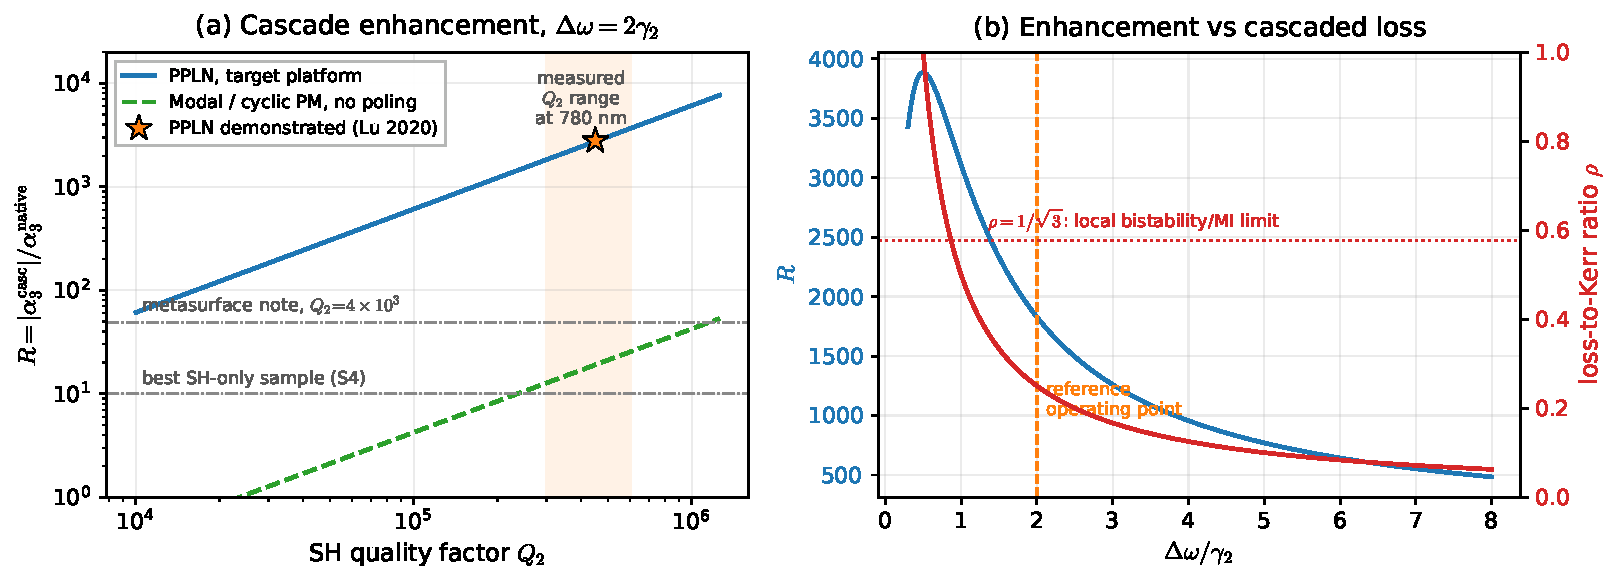
\includegraphics[width=\textwidth]{ring_R_landscape.pdf}
  \caption{(a) Cascaded enhancement $R$ versus SH quality factor at the
  reference operating point $\Dom=2\gamma_2$, for the poled and unpoled
  designs, with the demonstrated device marked.  The horizontal
  reference lines are the metasurface note's $R\simeq12$ at
  $Q_2=4\times10^3$ and the best fabricated SH-only sample
  ($R^{(1\mathrm R)}=2.5$).  (b) The operating-point trade-off: $R$ falls
  as $1/\Dom$ while the cascaded loss-to-Kerr ratio $\rho$ falls at the
  same rate, and bistability is lost above $\rho=1/\sqrt3$.}
  \label{fig:Rlandscape}
\end{figure}

\subsection{Numbers}

\begin{table}[H]
\centering
\small
\begin{tabular}{lrrrrrr}
\toprule
design & $g/2\pi$ & $Q_2$ & $R$ & $\Ucasc/2\pi$
 & $P_{\text{bist}}$ & $P_{\text{MI}}$\\
 & [MHz] & & & [Hz/ph] & [$\mu$W] & [$\mu$W]\\
\midrule
A: PPLN demonstrated & $1.20$ & $4.5\!\times\!10^5$ & $2796$ & $-1587$ & $72.8$ & $20.3$\\
B: PPLN target       & $1.42$ & $3.0\!\times\!10^5$ & $1828$ & $-1472$ & $36.6$  & $8.4$\\
C: no poling         & $0.12$ & $3.0\!\times\!10^5$ & $13$   & $-10$   & $7039$& $1216$\\
\midrule
native Kerr, same ring & --- & --- & $1$ & $+0.80$ & $14405$ & $9357$\\
\bottomrule
\end{tabular}
\caption{Cascaded response at cold-cavity $\Dom=2\gamma_2$.  The
bistability column is the exact threshold, minimised over pump detuning
with the cascaded coefficients evaluated at the pump-frame mismatch
$\Delta_{\text{eff}}=\Dom-2\delta_1$ (Section~\ref{sec:bist}); the
parametric column is the multimode Bogoliubov threshold of
Section~\ref{sec:comb} at $D_2/2\pi=10$~MHz.  The native row uses the
Design~B ring with the SH detuned away; its parametric entry is the
standard single-sideband-pair Kerr estimate.}
\label{tab:summary}
\end{table}

\paragraph{The SH coupling condition is a free $2\times$.}  Table~\ref{tab:designs}
takes $Q_2^{\text{load}}=3\times10^5$ with $Q_2^{\text{int}}=6\times10^5$,
i.e.\ a critically coupled SH.  The cascade does not need the SH
extracted --- it needs it \emph{stored} --- so leaving the SH port
under-coupled raises $Q_2^{\text{load}}$ toward $Q_2^{\text{int}}$ and
$R$ with it, to $3.7\times10^3$ in the fully under-coupled limit.  The
price is that the SH power is then dissipated internally rather than
carried off chip, which doubles the cascade's own heat load
(Section~\ref{sec:competing}), and that $g$ can no longer be calibrated
on that device.  The headline numbers below keep the conservative
critically coupled choice.

For Design~B the equivalent material parameters are
\begin{equation}
  n_2^{\text{eff}}=-3.3\times10^{-16}\ \mathrm{m^2/W},\qquad
  \chithree_{\text{eff}}=-5.7\times10^{-18}\ \mathrm{m^2/V^2},
\end{equation}
i.e.\ a self-defocusing nonlinearity three orders of magnitude above
native LN and comparable to the largest reported non-resonant material
Kerr coefficients --- but, unlike those, sign-tunable and available in a
low-loss, TPA-free host at telecom.

\paragraph{Consistency with the metasurface note.}  Inverting the main
note's boxed result
$\chithree_{\text{casc}}=-\omega_1|\chitwo|^2\eta_{\text{geom}}/(6n_2^2\Dom)$
with the numbers above returns $\eta_{\text{geom}}=0.93$ for Design~B
and $0.006$ for Design~C.  The unpoled value is squarely in the range
found for the fabricated metasurface samples ($0.01$--$0.04$); the
poled value sits at the physical ceiling $\eta_{\text{geom}}\le1$, which
is again the prefactor question of Section~\ref{sec:anchor} (on the
larger-prefactor branch it becomes $\simeq0.23$, a comfortable value for
quasi-phase-matched interaction).  Either way the ordering is the
message: \textbf{periodic poling over a full circumference is what a
metasurface meta-atom cannot do}, and it is worth a factor of $\sim100$
in $R$.

% =======================================================================
\section{Design rules specific to the ring}\label{sec:rules}

\subsection{Rule 1: the cascade costs no bandwidth here}\label{sec:rule1}

In the metasurface, $\gamma_2<\gamma_1$ and the useful bandwidth was
$\min(\gamma_1,\gamma_2)=\gamma_2$: the cascade was the bottleneck, and
the sum rule of note \S7 bit immediately.  In a ring,
\begin{equation}
  \frac{\gamma_2}{\gamma_1}=\frac{\omega_2/Q_2}{\omega_1/Q_1}
     =\frac{2Q_1}{Q_2}\;\simeq\;6.7\quad\text{(Design B)} ,
\end{equation}
so the SH is far broader than the FM and the FM cavity remains the
bottleneck, exactly as it would be for a native-Kerr ring.

A susceptibility argument makes the scale plausible --- a modulation of
$|a|^2$ at $\Omega$ drives the SH through
$[i(\delta_2-\Omega)+\kappa_2]^{-1}$, so the cascaded coefficient is
obtained from \eqref{eq:Ucasc} by $\Dom\to\Dom+\Omega$, rolling off at
$|\Dom|/2\pi=2.6$~GHz against $\kappa_1/2\pi=97$~MHz --- but a
susceptibility scale is not a transfer function.  We therefore computed
the actual small-signal response: linearise the driven system
\eqref{eq:cmt-a}--\eqref{eq:cmt-b} about its CW fixed point and solve
$(-i\Omega\mathbb{1}-J)\,\delta y=\hat p$ for a modulation of the input
power, with the drive perturbation taken along $p$ (not along the real
axis --- with $a$ gauged real, $p=\sqrt n[(\kappa_1+\kcasc n)
+i(\delta_1-Un)]$).  The reference is a \emph{matched} single-mode
cavity: same photon number, same total per-photon Kerr
$\Unat+\Ucasc$, same nonlinear loss $\kcasc$, but responding
instantaneously.  Any difference is then attributable solely to the
SH's finite response time.

At $20\,\mu$W and $\Dom=2\gamma_2$ the cascade's $3$~dB bandwidth is
$421$~MHz against $454$~MHz for the matched instantaneous reference:
\textbf{the SH costs $7\%$ of modulation bandwidth}, and $2\%$ at
$2\,\mu$W.  Equivalently, the four eigenvalues of the full Jacobian
separate cleanly into an FM-like pair at $|\lambda|=2.45\,\kappa_1$ and
an SH-like pair at $|\lambda|=29.6\,\kappa_1$, a factor $12$ apart.
The resonator, not the cascade, sets the speed.
Figure~\ref{fig:validation}(b) shows both curves.

\subsection{Rule 2: locality of the cascaded response}\label{sec:rule2}

The exact elimination of the SH in the time domain is
\begin{equation}
  b(t)=-ig\!\int_0^\infty\! e^{-(\kappa_2+i\delta_2)\tau}\,a^2(t-\tau)\,d\tau ,
  \label{eq:bmemory}
\end{equation}
so the memory kernel decays at the rate $\kappa_2$ but \emph{oscillates}
at $\delta_2$.  What controls whether the response may be treated as
instantaneous is the modulus
\begin{equation}
  \boxed{\;\Omega_{\text{env}}\;\ll\;\sqrt{\kappa_2^{2}+\delta_2^{2}}\;}
  \label{eq:locality}
\end{equation}
where $\Omega_{\text{env}}$ is the bandwidth of the FM envelope, not
$\kappa_2$ alone.  Detuning helps: at the reference operating point
$\delta_2=-2\gamma_2=-4\kappa_2$, so the right-hand side is
$\sqrt{17}\,\kappa_2=27.5\,\kappa_1$, four times more forgiving than the
naive $\kappa_2/\kappa_1=6.7$.

A crude reading of \eqref{eq:locality} with
$\Omega_{\text{env}}\sim\kappa_1$ and $\delta_2\to0$ would give
$Q_2\lesssim2Q_1$; we quote \eqref{eq:locality} instead, because that
inequality is not a general boundary and is unnecessarily pessimistic
wherever the device is actually operated.  The measured consequence is
the $7\%$ bandwidth cost of Section~\ref{sec:rule1}.  What does remain
true is the qualitative trade: $R\propto Q_2$ wants a narrow SH
resonance, locality wants a broad one, and the two meet near
$Q_2\sim Q_1$.  Far beyond that the dynamics ceases to be Kerr-like and
one is in the quadratic-soliton regime.

\subsection{Rule 3: the local loss-to-Kerr limit
\texorpdfstring{$\rho<1/\sqrt3$}{rho < 1/sqrt3}}\label{sec:rule3}

Using \eqref{eq:effective}, the CW steady state satisfies
\begin{equation}
  |p|^2=n\Bigl[(\kappa_1+\kcasc n)^2+(\delta_1-U n)^2\Bigr],
  \qquad |p|^2=\frac{2\kappa_{1,\text{ex}}P_{\text{in}}}{\hbar\omega_1},
  \label{eq:cubic}
\end{equation}
a cubic in $n$.  Turning points require the discriminant of
$dP/dn=3(U^2+\kcasc^2)n^2+4(\kappa_1\kcasc-\delta_1U)n+(\delta_1^2+\kappa_1^2)$
to be positive, i.e.
\begin{equation}
  4(\rho-s)^2>3(1+\rho^2)(s^2+1),\qquad s\equiv|\delta_1|/\kappa_1 ,
  \label{eq:bist-cond}
\end{equation}
with the pump on the side the resonance moves toward,
$\operatorname{sign}\delta_1=\operatorname{sign}U$.  As $s\to\infty$ this
requires $4>3(1+\rho^2)$, i.e.
\begin{equation}
  \boxed{\;\rho<\frac{1}{\sqrt3}\simeq0.577
   \quad\Longleftrightarrow\quad
   |\Delta_{\text{eff}}|>\frac{\sqrt3}{2}\,\gamma_2\simeq0.87\,\gamma_2\;}
  \label{eq:rule3}
\end{equation}
Equation~\eqref{eq:bist-cond} also raises the required pump detuning:
$|\delta_1|/\kappa_1$ grows from $\sqrt3=1.73$ at $\rho=0$ to $3.50$ at
$\rho=1/4$ and diverges as $\rho\to1/\sqrt3$.  This is the cascaded
analogue of the requirement that the two-photon figure of merit be small
enough for Kerr bistability, and the same inequality reappears in
Section~\ref{sec:comb} as the single-sideband-pair parametric condition.

\paragraph{It is a condition on $\Delta_{\text{eff}}$, not on the cold
cavity.}  This distinction is easy to get wrong and we got it wrong in
an earlier draft.  The coefficients $U$ and $\kcasc$ must be evaluated
at the \emph{pump-frame} mismatch $\Delta_{\text{eff}}=\Dom-2\delta_1$
of \eqref{eq:delta2}, which moves as the pump is scanned.  Freezing them
at the cold-cavity $\Dom$ turns \eqref{eq:rule3} into an apparent
fabrication requirement $|\Dom|>0.87\gamma_2$, and that is
\textbf{false}: the experimenter chooses $\delta_1$, and a pump detuned
far enough to one side supplies whatever $\Delta_{\text{eff}}$ is needed.
Solving the threshold problem exactly --- minimising the fold power over
$\delta_1$ with $U(\Delta_{\text{eff}})$ and $\kcasc(\Delta_{\text{eff}})$
--- gives a threshold that is finite for \emph{every} cold-cavity
detuning, including $\Dom=0$, where it is $304\,\mu$W.  The frozen model
diverges there (Figure~\ref{fig:thresholds}(b)).  What survives of
Rule~3 is a genuine local statement: at the operating point, the
pump-frame loss-to-Kerr ratio must satisfy $\rho<1/\sqrt3$.

% =======================================================================
\section{Branch stability and the dispersive-breakdown scale}\label{sec:ceiling}

The main note's saturation criterion $|\beta a_1|\to|\Dom|$ translates,
via \eqref{eq:g-beta}, into $\sqrt2\,g\sqrt n=|\Dom|$, i.e.
\begin{equation}
  n_{\text{sat}}=\frac{\Dom^2}{2g^2},
  \qquad\text{whence}\qquad
  |\Ucasc|\,n_{\text{sat}}\simeq|\Dom| .
  \label{eq:nsat}
\end{equation}
\emph{The cascaded resonance shift reaches order $\Dom$ itself} at this
scale, which is $4\kappa_2/\kappa_1=8Q_1/Q_2$ FM linewidths.  It should
be read as the point at which the coherent SH coupling stops being a
small perturbation on the detuning --- a dispersive-breakdown scale ---
not as an exact saturation of the equations of motion.  The steady-state
elimination \eqref{eq:bss} remains algebraically exact at any amplitude;
what fails beyond this scale is the interpretation of the result as a
weak, local Kerr nonlinearity.

We checked \eqref{eq:nsat} against a direct linear-stability analysis:
linearising \eqref{eq:cmt-a}--\eqref{eq:cmt-b} about the CW fixed point
(with $a$ real by gauge, $b$ from \eqref{eq:bss}) gives a $4\times4$ real
Jacobian whose largest eigenvalue real part crosses zero at a critical
photon number $n_c$.  Over $\Dom/\gamma_2\in[0.6,8]$ the numerical
$n_c$ exceeds $n_{\text{sat}}$ by a factor $1.13$--$1.92$ (median
$1.14$), so \eqref{eq:nsat} is a mildly conservative estimate and the
scaling is correct.  Figure~\ref{fig:stability} shows both.

For Design~B at $\Dom=2\gamma_2$ this is $n_c=2.0\times10^6$ photons,
$153\,\mu$W of input power, and a resonance shift of $30\,\kappa_1$ ---
an order of magnitude above the $\sqrt3\,\kappa_1$ needed for
bistability and the $1\,\kappa_1$ needed for switching.  Two
qualifications: the scan is along the $\delta_1=0$ path and the
Jacobian used here omits the native Kerr (which is $10^{-3}$ of the
cascaded term), and the loss of stability of \emph{this} branch does not
imply that no CW state exists.  With those caveats,
\textbf{dynamic range is not the limiting factor}; thermal and
photorefractive effects (Section~\ref{sec:competing}) reach that
territory first.

\begin{figure}[H]
  \centering
  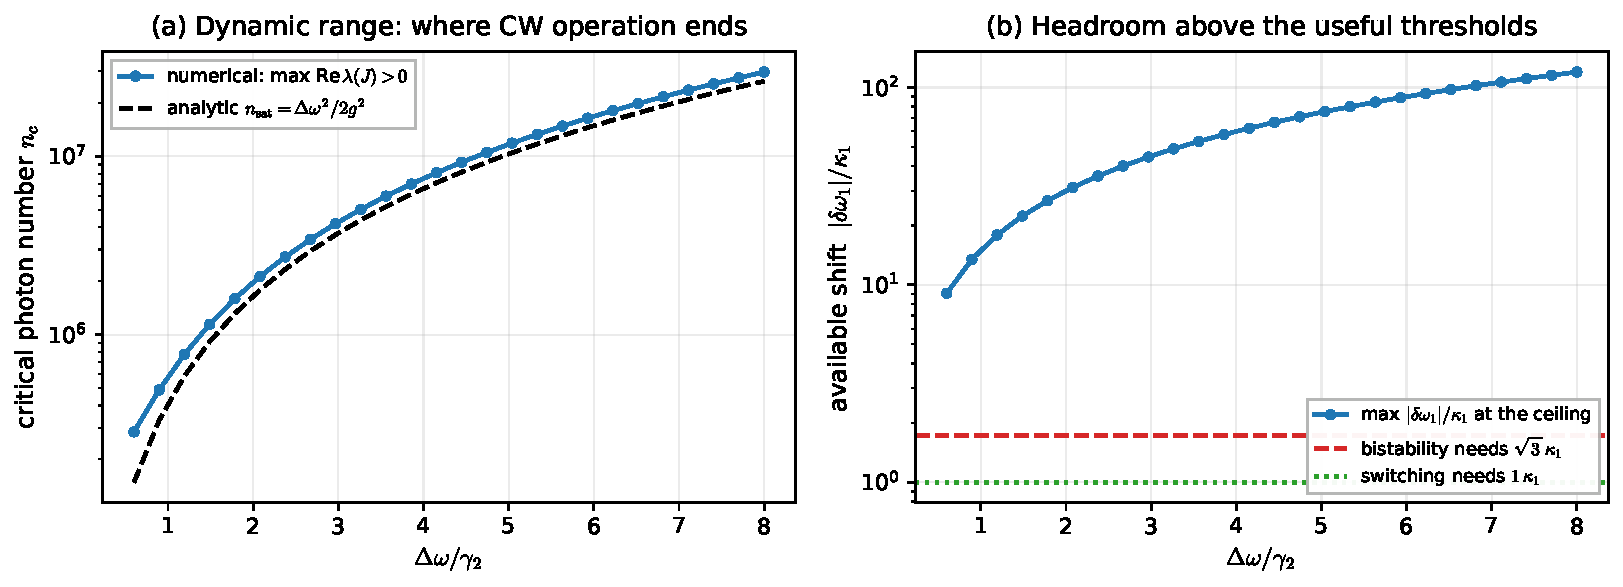
\includegraphics[width=\textwidth]{ring_stability.pdf}
  \caption{(a) Critical photon number from the $4\times4$ Jacobian
  compared with the analytic ceiling $n_{\text{sat}}=\Dom^2/2g^2$.
  (b) The resonance shift available at that ceiling, in FM linewidths,
  against the shifts required for bistability and for switching.}
  \label{fig:stability}
\end{figure}

% =======================================================================
\section{Observables}\label{sec:observables}

\subsection{Sign-tunable Kerr: the primary signature}\label{sec:signflip}

The cleanest demonstration is not a large nonlinearity --- large
nonlinearities can be mimicked by thermal and photorefractive effects ---
but a nonlinearity that \emph{changes sign} under a control the
competing mechanisms do not respond to.  From \eqref{eq:Ucasc}, walking
the SH resonance through $2\omega_1$ takes the FM resonance shift from
red ($\Dom<0$, self-focusing) through zero to blue ($\Dom>0$,
self-defocusing), with extrema at $\Dom=\mp\kappa_2$ of magnitude
$g^2/\kappa_2$.  Native LN Kerr, thermal shifts and photorefractive
shifts are all one-signed.

\begin{figure}[H]
  \centering
  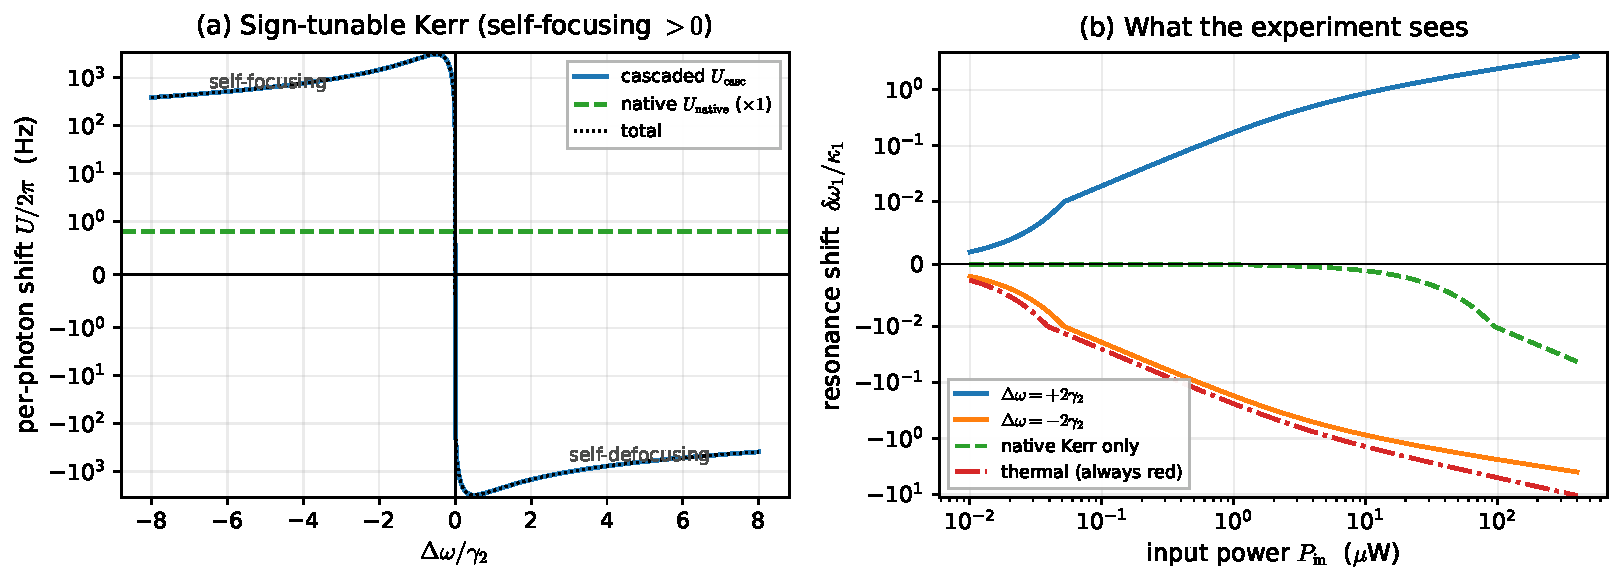
\includegraphics[width=\textwidth]{ring_sign_flip.pdf}
  \caption{(a) Per-photon Kerr coefficient versus SH detuning
  (Design~B): the cascade is odd in $\Dom$ and dwarfs the native
  contribution over the whole useful range.  (b) The corresponding FM
  resonance shift versus input power, with $n$ computed
  self-consistently (including the cascaded loss and self-detuning), for
  both signs of $\Dom$, against the native-Kerr and thermal
  backgrounds.  A blue shift is a strong indicator of the cascade, but not
  by itself proof: photorefraction in thin-film LN can also shift a
  resonance blue (Section~\ref{sec:competing}).  The decisive test is the
  controlled reversal under $\Dom\to-\Dom$.}
  \label{fig:signflip}
\end{figure}

\paragraph{How to sweep $\Dom$.}  Two knobs, both native to LN:
\begin{itemize}[leftmargin=1.6em,itemsep=2pt]
\item \textbf{Temperature.}  Each resonance tunes fast
  ($d\omega_1/dT\simeq-2\pi\times2.8$~GHz/K and
  $d\omega_2/dT\simeq-2\pi\times5$--$7$~GHz/K), but $\Dom=2\omega_1-\omega_2$
  is a \emph{difference} of two nearly equal quantities and therefore
  tunes slowly.  Its rate depends on the dispersion of $dn/dT$ between
  $1.55\,\mu$m and $775$~nm, which is not well pinned: taking
  $(dn/dT)_{\text{SH}}=3.3$--$4.5\times10^{-5}$~K$^{-1}$ against
  $3.3\times10^{-5}$ at the FM gives
  $d\Dom/dT$ anywhere from $-0.34$ to $+1.6$~GHz/K.  \emph{Both the sign
  and the magnitude must be measured}, but in every case the scale is
  $\sim\gamma_2$ per few kelvin: sweeping $\Dom$ over $\pm2\gamma_2$
  takes $2$--$9$~K.  The near-cancellation is a gift --- $\Dom$ is a
  coarse-grained, easily stabilised coordinate even though each
  resonance individually is not.
\item \textbf{Electro-optic (the important one).}  With $r_{33}=30.8$~pm/V
  at the FM and $34$~pm/V at the SH, the same difference structure gives
  $d\Dom/dE=-2\pi\times3.0$~GHz per V/$\mu$m: already $2.4\,\gamma_2$ at
  $1$~V/$\mu$m, $4.7\,\gamma_2$ at $2$~V/$\mu$m and $23\,\gamma_2$ at
  $10$~V/$\mu$m.  Modulator-level drive voltages therefore sweep $\Dom$
  across several SH linewidths, and the Pockels effect supports tens of
  GHz of modulation bandwidth in this platform, so $\Dom$ can be dithered
  far faster than any thermal or photorefractive response.  This is the
  single most useful thing lithium niobate contributes beyond its
  $\chitwo$.
\end{itemize}

\subsection{Bistability and threshold power}\label{sec:bist}

Solving \eqref{eq:cubic} exactly --- minimising the fold power over
$\delta_1$ with the coefficients taken at
$\Delta_{\text{eff}}=\Dom-2\delta_1$, as Section~\ref{sec:rule3}
requires --- gives the hysteresis loops of
Figure~\ref{fig:bistability}.  For Design~B the threshold falls from
$14.4$~mW (native, where there is no $\Delta_{\text{eff}}$ dependence and
the closed form is exact) to $36.6\,\mu$W at cold $\Dom=2\gamma_2$, a
factor $394$.  Note this is \emph{less} than $R=1828$: the cascaded
two-photon loss costs roughly a factor $5$, both by forcing a larger
pump detuning (Rule~3) and by broadening the resonance.  The
fixed-coefficient treatment overestimates the threshold by $26\%$ here
($46\,\mu$W) and diverges as $\Dom\to\tfrac{\sqrt3}{2}\gamma_2$, where
the exact answer stays finite.

It is worth being blunt about what the native column of
Table~\ref{tab:summary} means.  At the $14.4$~mW required for native
Kerr bistability, the lumped thermal model of
Section~\ref{sec:competing} predicts a thermal shift of
$\sim1.4\times10^3$ linewidths.  \textbf{Native Kerr bistability is not
merely harder in this ring, it is thermally inaccessible by three orders
of magnitude}; the cascade does not just improve the number, it is what
makes the observable exist at all.  Optimising over the
operating point (Figure~\ref{fig:thresholds}(b)) gives
\begin{equation}
  \Dom^{\text{opt}}\simeq3.3\,\gamma_2,\qquad
  P_{\text{bist}}=31.7\,\mu\mathrm{W},
  \qquad\text{at }\delta_1=-2.4\,\kappa_1,\ \
  \Delta_{\text{eff}}=3.7\,\gamma_2,
\end{equation}
a shallow optimum arising because $R\propto1/\Dom$ pushes one way while
$\rho\propto1/\Dom$ pushes the other.  (The frozen model's apparent
optimum of $3.7\gamma_2$ was in fact the \emph{pump-frame} mismatch at
the true optimum, which is why it looked numerically reasonable.)  We
therefore recommend a cold-cavity $\Dom\simeq3\gamma_2$ rather than the
metasurface note's $2\gamma_2$ for any threshold-limited experiment.

The transmission lineshape is the direct observable:
Figure~\ref{fig:bistability}(b) shows the resonance tilting to opposite
sides for $\Dom=\pm2\gamma_2$ at $30\,\mu$W.  \emph{The tilt reversal
under a sign change of $\Dom$, at fixed power, is the measurement.}

\begin{figure}[H]
  \centering
  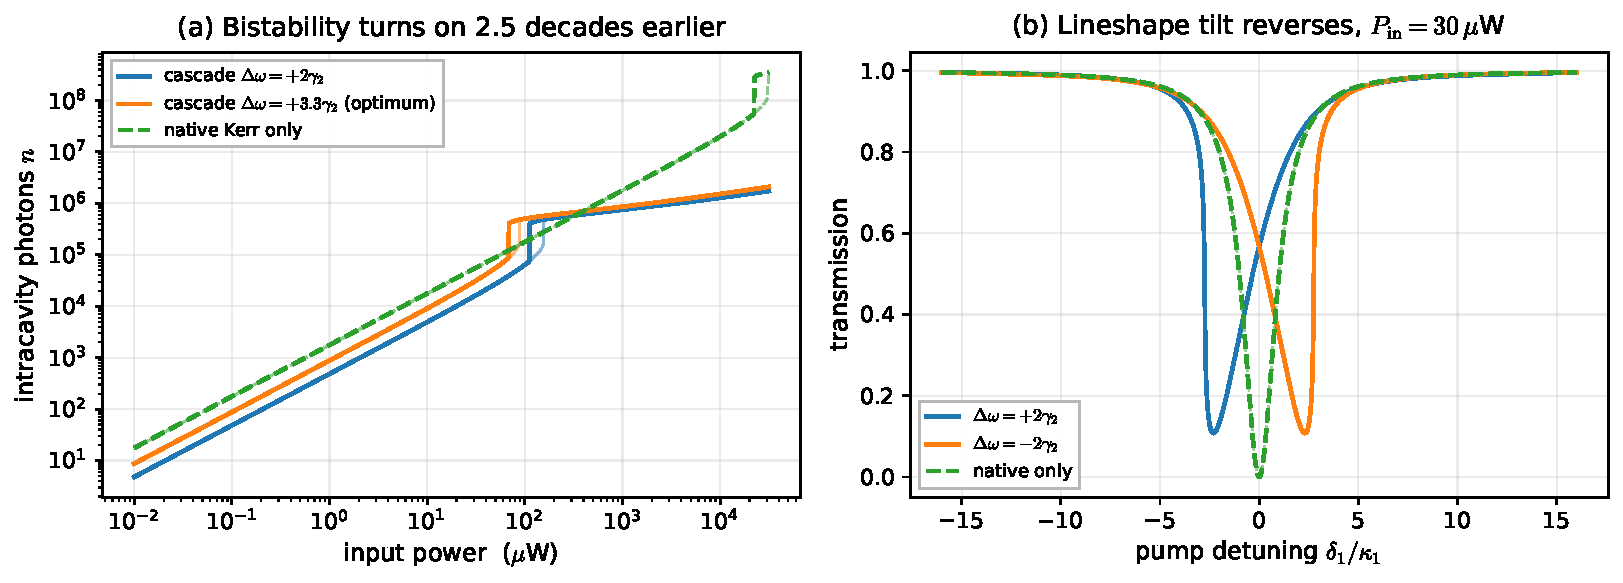
\includegraphics[width=\textwidth]{ring_bistability.pdf}
  \caption{(a) Steady-state intracavity photon number versus input power
  for the cascade at two operating points and for the native Kerr, each
  at $1.45\times$ its own minimum bistable detuning.  The $-\Dom$
  branches give identical $|n|$ curves and are not drawn.  (b)
  Transmission lineshapes at $30\,\mu$W: the tilt reverses with the sign
  of $\Dom$ while the native response stays nearly symmetric.}
  \label{fig:bistability}
\end{figure}

\begin{figure}[H]
  \centering
  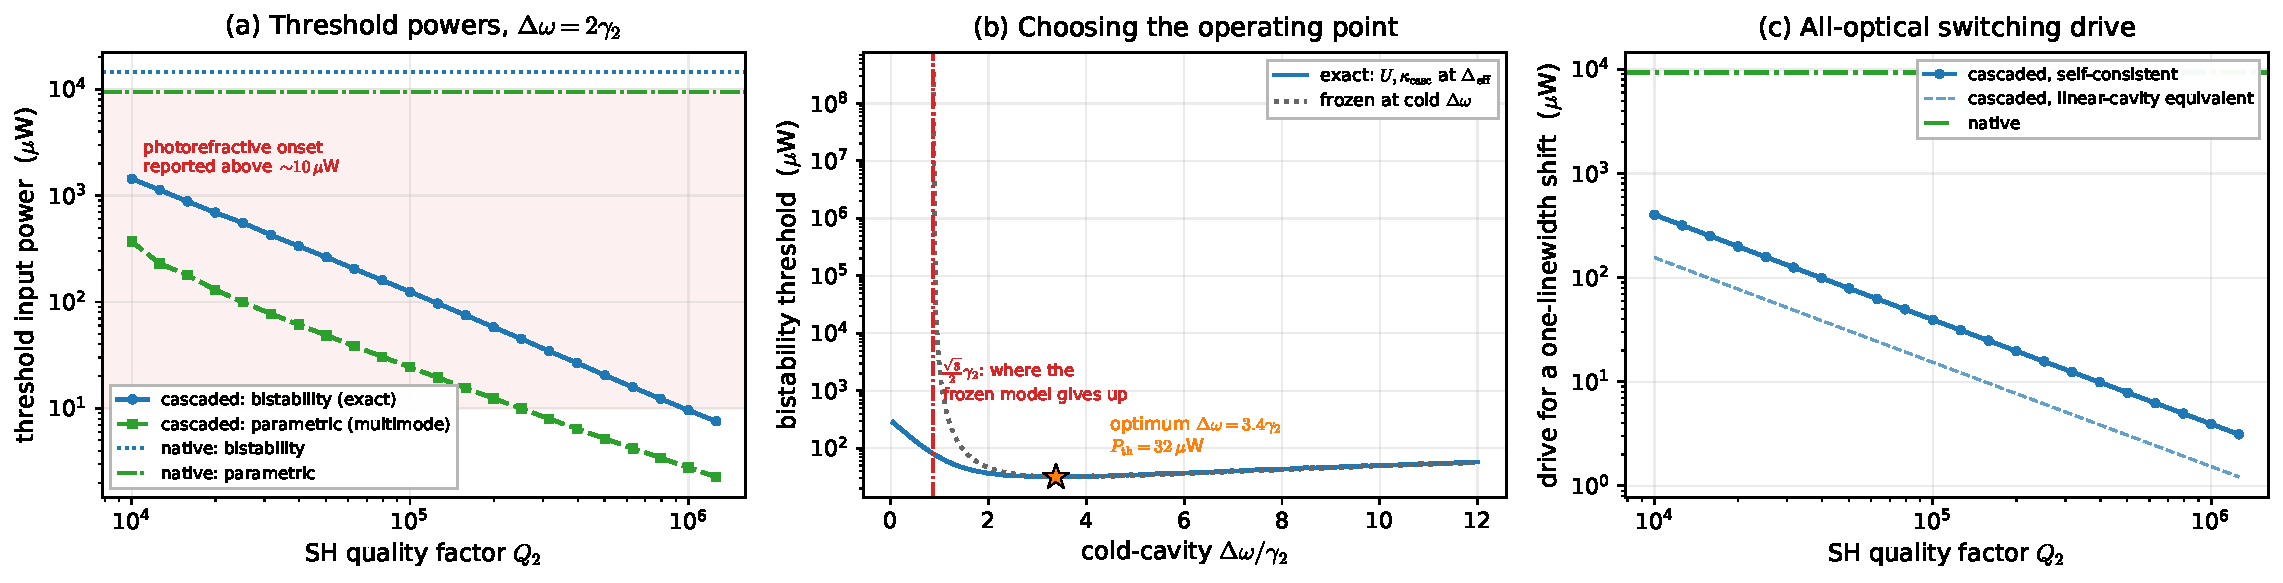
\includegraphics[width=\textwidth]{ring_thresholds.pdf}
  \caption{(a) Bistability and parametric thresholds versus $Q_2$,
  cascaded and native, with the photorefractive onset reported in
  Ref.~\cite{Lu2020} shaded.  (b) Threshold versus operating point,
  showing the shallow optimum near $\Dom\simeq3.7\gamma_2$ and the
  divergence at $\Dom=\tfrac{\sqrt3}{2}\gamma_2$; the dotted curve is
  the idealisation with the cascaded loss switched off, whose gap to the
  solid curve is the price of $\rho$.  (c) Drive power and intracavity
  energy for a one-linewidth shift.}
  \label{fig:thresholds}
\end{figure}

\subsection{Self- and cross-phase modulation, and switching}

The per-photon shift \eqref{eq:Ucasc} is self-phase modulation.  For
cross-phase modulation between two FM modes $a_1,a_2$, the mediating SH
mode is the one at the \emph{sum} azimuthal number, and the interaction
Hamiltonian carries the usual non-degenerate factor,
$\hat H/\hbar\supset2g(a_1^\dagger a_2^\dagger c+\text{h.c.})$.
Eliminating $c$ gives an XPM coefficient
\begin{equation}
  U_{\text{XPM}}=-\frac{4g^2\Dom_c}{\Dom_c^2+\kappa_2^2}=2\,\Ucasc(\Dom_c),
\end{equation}
i.e.\ the familiar factor-of-two XPM/SPM ratio of an ordinary Kerr
medium, but evaluated at the detuning $\Dom_c$ of \emph{that} SH mode,
which is generally different (Section~\ref{sec:comb}).  The factor is
exactly two only if the two triplets share the same three-wave overlap,
$g_{12c}=g_{11b}$; in a real ring they differ through the frequencies,
transverse profiles, tensor projections and QPM overlap, so read it as
``two, up to the overlap ratio''.

For switching, the relevant figure is the drive needed for a
one-linewidth shift, $n_{\text{sw}}=\kappa_1/|U|$:
\begin{center}
\small
\begin{tabular}{lrr}
\toprule
 & cascaded (B, $\Dom=2\gamma_2$) & native \\
\midrule
photons for $\delta\omega_1=\kappa_1$ & $6.6\times10^4$ & $1.2\times10^8$\\
intracavity switching energy          & $8.4$~fJ        & $15.4$~pJ\\
linear-cavity-equivalent loading      & $5.1\,\mu$W     & $9.4$~mW\\
self-consistent CW drive, $\delta_1=0$& $13.1\,\mu$W    & $18.7$~mW\\
self-consistent, optimal retuning     & $7.6\,\mu$W     & ---\\
\bottomrule
\end{tabular}
\end{center}
The distinction in the last three rows matters.  The intracavity energy
is the clean figure of merit.  The ``linear-cavity-equivalent'' row
inverts the \emph{linear} loading formula and is what a naive estimate
returns; it understates the real drive by $2.6\times$, because at the
switching point the resonance has already moved by a full linewidth and
the cavity is no longer being driven on resonance.  The self-consistent
rows solve \eqref{eq:cubic} for the power that actually reaches
$n_{\text{sw}}$.
The cascade brings all-optical switching in LN from the ``needs an
amplifier'' regime into the ``needs a laser diode'' regime, at a
switching energy competitive with the best resonant Kerr switches, and
with a switching \emph{speed} limited by $\kappa_1$ rather than by the
nonlinearity (Rule~1).

\subsection{Parametric oscillation and frequency combs}\label{sec:comb}

The degenerate four-wave-mixing process $2a_p\to a_s+a_i$ with
$m_s+m_i=2m_p$ is mediated by the \emph{same} SH mode that produces the
pump's SPM, so it inherits the full cascaded coupling.  A
gain-equals-loss estimate is not adequate here, so we solve the
linear-stability problem properly.

\paragraph{Multimode Bogoliubov threshold.}  Retain the pump $a_0$, a
sideband pair $a_\pm$ at $m_p\pm q$, the SH mode $b_0$ at $2m_p$ driven
by the pump, and the SH sidebands $b_\pm$ at $2m_p\pm q$:
\begin{equation}
  \hat H/\hbar\supset g\bigl(a_0^{\dagger2}b_0\bigr)
   +2g\bigl(a_+^\dagger a_-^\dagger b_0\bigr)
   +2g\bigl(a_0^\dagger a_+^\dagger b_+\bigr)
   +2g\bigl(a_0^\dagger a_-^\dagger b_-\bigr)+\text{h.c.}
\end{equation}
Linearising about the CW pump closes a $4\times4$ system in
$(\delta a_+,\delta a_-^*,\delta b_+,\delta b_-^*)$ whose largest
eigenvalue real part gives the parametric gain; the threshold is the
lowest input power at which it turns positive, minimised over $\delta_1$
and $q$.  The parametric gain enters through $b_0$, while the
pump-induced cross-phase shift and cascaded loss on the sidebands enter
through $b_\pm$, whose detunings walk off with $q$ because the FM and SH
free spectral ranges differ.  (This assumes equal modal overlaps for
every triplet, and neglects the native Kerr on the sidebands, which is
$\sim10^{-3}$ of the cascaded term.)

For Design~B this gives $P_{\text{MI}}=8.4\,\mu$W against $9.4$~mW
natively, a factor $1100$.  The result is insensitive to the ring
dispersion --- $8.1$, $8.1$ and $8.4\,\mu$W for
$D_2/2\pi=1$, $10$ and $50$~MHz --- because the instability simply
selects whichever $q$ brings the sideband into resonance.  For reference,
the single-mode gain-equals-loss estimate gives $6.8\,\mu$W and its
self-consistent version $12.1\,\mu$W, so the heuristics bracket the
answer to within a factor of $1.5$ but neither is reliable on its own.

\paragraph{The local single-pair condition.}  Adiabatically eliminating
$b_\pm$ when they are degenerate with $b_0$ (no walk-off) reduces the
$4\times4$ to $\bigl[\begin{smallmatrix}A&B\\ B^*&A^*\end{smallmatrix}\bigr]$
with $A=-(i\delta_q+\kappa_1)+2iUn-2\kcasc n$ and $B=iUn-\kcasc n$,
whose eigenvalues are $\operatorname{Re}A\pm\sqrt{|B|^2-(\operatorname{Im}A)^2}$.
Instability at the optimal sideband detuning $\delta_q=2Un$ requires
$n|U|\sqrt{1+\rho^2}>\kappa_1+2\rho|U|n$, i.e.
\begin{equation}
  n_{\text{MI}}=\frac{\kappa_1}{|U|\bigl(\sqrt{1+\rho^2}-2\rho\bigr)},
  \qquad\text{possible only for }\ \rho<\frac{1}{\sqrt3},
  \label{eq:mi-local}
\end{equation}
\emph{the same $\rho<1/\sqrt3$ that governs bistability}
(Section~\ref{sec:rule3}).  The $4\times4$ reproduces
\eqref{eq:mi-local} to $9\times10^{-4}$ in the zero-walk-off limit,
which is how we validated it.  With walk-off the SH sidebands are pushed
off resonance, the cross-phase term is suppressed, and the constraint on
$\rho$ relaxes --- one reason the full calculation is needed.

Two ring-specific consequences:

\paragraph{An extra degree of freedom for dispersion engineering.}
Modulation instability of the bright-soliton kind requires
$\beta_2\gamma_{\text{NL}}<0$, and native LN is self-focusing.  It would
be too strong to say that combs therefore \emph{demand} anomalous
dispersion --- normal-dispersion microresonators support coherent dark-pulse
(platicon) states, and those are routinely generated~\cite{Kippenberg2018}.
The defensible claim is narrower: a sign-tunable $\chithree$ adds a
degree of freedom to MI and phase-matching engineering that a fixed-sign
Kerr medium does not have, and in particular lets the \emph{same} ring
be operated in either MI regime by moving $\Dom$.  A related capability
is nulling: at the $\Dom$ where $\Ucasc=-\Unat$ the total Kerr vanishes,
giving a Kerr-free high-$Q$ LN ring.

\paragraph{But the cascade is not a uniform $\chithree$ across the comb.}
Sum-frequency generation of FM lines $(m_p+q_1,m_p+q_2)$ lands on the SH
mode $2m_p+j$ with $j=q_1+q_2$, whose detuning walks off as
\begin{equation}
  \Dom_j=\Dom-j(\Omega_2-\Omega_1),
  \qquad
  \Omega_2-\Omega_1=\Omega_1\Bigl(\frac{n_{g,1}}{n_{g,2}}-1\Bigr)
  =-2\pi\times25.4\ \mathrm{GHz}
\end{equation}
for Design~B, which is $19.7\,\gamma_2$ \emph{per mode index}.  Only
$j=0$ --- which covers the pump SPM and the degenerate parametric
process above --- is resonant; $j=\pm1$ is already suppressed tenfold
(Figure~\ref{fig:quantum}(b)).  So the parametric \emph{threshold}
reduction is rigorous, but the subsequent comb dynamics is not
Lugiato--Lefever-like, because XPM among comb lines is strongly
mode-selective.  This is the same physics that distinguishes quadratic
combs from Kerr combs in the literature~\cite{QuadraticComb2024}.
Making the cascade broadband requires group-index matching: keeping
$|\Dom_j|$ within a factor of a few of $|\Dom|$ out to $|j|=J$ needs
$|\Delta n_g|/n_g\lesssim\Dom/(J\,\Omega_1)$, which is
$6\times10^{-4}$ for $J=10$ at this operating point and scales as $1/J$.
The number is therefore tied to a chosen comb span, not universal.  It
is a demanding but well-posed dispersion-engineering target and, in our
view, the most interesting design question this analysis raises.

\subsection{Single-photon anharmonicity: the cascade is the wrong regime}

For photon blockade one needs a per-photon anharmonicity comparable to or
exceeding the linewidth (the precise condition depends on the dressed-state
structure and the linewidths, so the ``$=1$'' line in
Figure~\ref{fig:quantum}(a) is schematic).  In the dispersive (cascaded) regime, with $\Dom\gtrsim\gamma_2=2\kappa_2$,
\begin{equation}
  \frac{|\Ucasc|}{\kappa_1}=\frac{2g^2}{|\Dom|\,\kappa_1}
   \;\lesssim\;\frac{g}{\kappa_1}\cdot\frac{g}{\kappa_2},
  \label{eq:blockade}
\end{equation}
the \emph{product} of two small numbers, whereas resonant operation
($\Dom\to0$, no Kerr description) has the single small number
$g/\kappa_1$ as its figure of merit.  For Design~B,
$|\Ucasc|/\kappa_1=1.5\times10^{-5}$ against $g/\kappa_1=1.5\times10^{-2}$.
\textbf{Cascading buys three orders of magnitude of classical
nonlinearity and loses three orders of magnitude of quantum
anharmonicity}, and the two statements are the same statement: the
cascade converts a strong resonant coupling into a weak dispersive one
in exchange for a Kerr-like, classically useful response.  Quantum work
on this platform should stay resonant --- which is what
Ref.~\cite{Lu2020} in fact pursues: it is a demonstration of resonant
$\chitwo$ single-photon anharmonicity (and a proposal for unconventional
blockade), not of the dispersive cascade analysed here.  We use it only
as the source of a measured $g$.

\begin{figure}[H]
  \centering
  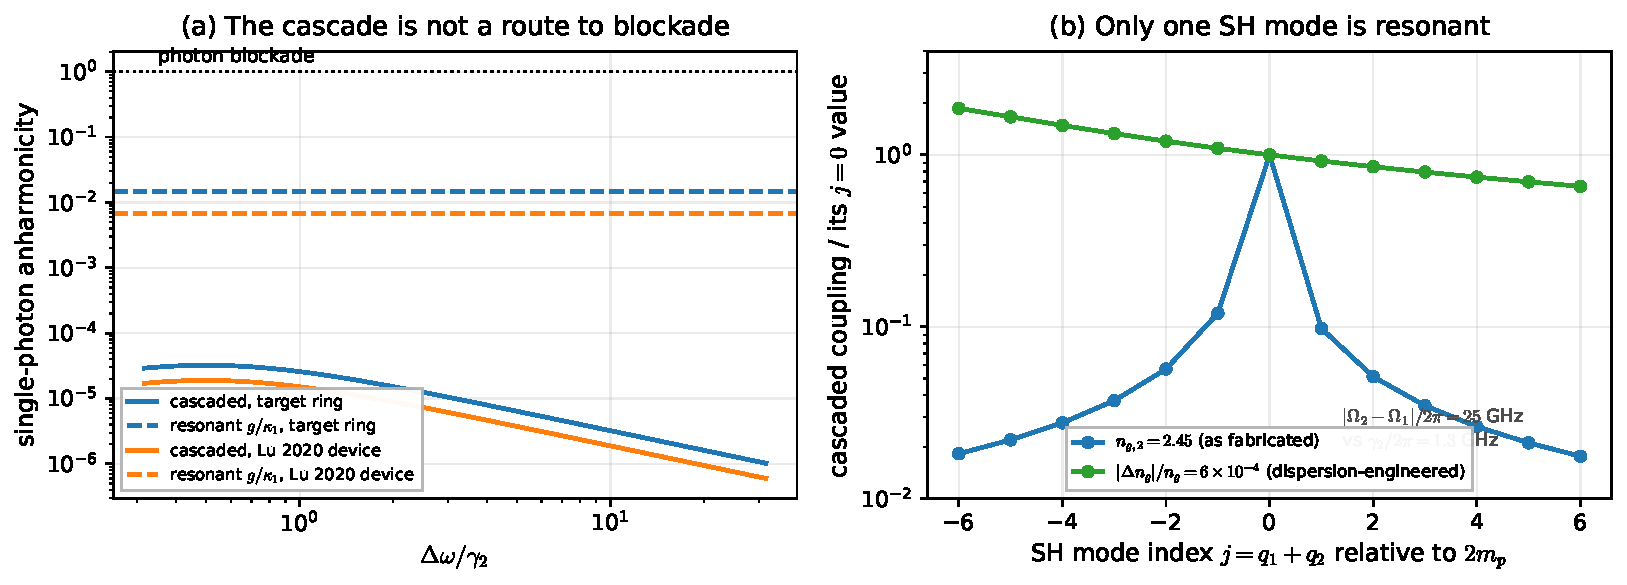
\includegraphics[width=\textwidth]{ring_quantum_comb.pdf}
  \caption{(a) Dispersive versus resonant single-photon figure of merit.
  (b) Cascaded coupling for the SH mode $2m_p+j$ relative to $j=0$: the
  FM/SH free-spectral-range walk-off detunes neighbouring SH modes by
  $\sim20\gamma_2$ per index, so only $j=0$ participates unless the group
  indices are matched.}
  \label{fig:quantum}
\end{figure}

% =======================================================================
\section{What actually competes: thermal and photorefractive shifts}
\label{sec:competing}

At the powers where the cascade produces a linewidth-scale shift
($\sim10\,\mu$W), two other mechanisms produce shifts of the same order.

\paragraph{Thermal.}  With
$dn/dT=3.3\times10^{-5}$~K$^{-1}$ and a thermal resistance
$R_{\text{th}}\sim3\times10^4$~K/W, the FM resonance red-shifts by
$|d\omega_1/dT|\,R_{\text{th}}P_{\text{abs}}$.  Getting $P_{\text{abs}}$
right requires care about bookkeeping.  The power leaving the FM through
the SH channel is $P_{\text{casc}}=2\hbar\omega_1\kcasc n^2$, but this is
not all local heat: only the fraction $\kappa_{2,0}/\kappa_2$ stays on
chip (the rest exits the SH port), and of that only the absorptive part
becomes heat rather than scattered light.  We therefore take
\begin{equation}
  P_{\text{abs}}=f_{\text{abs}}\Bigl[\,
     \underbrace{2\hbar\omega_1\kappa_{1,0}n}_{\text{FM intrinsic}}
     +\frac{\kappa_{2,0}}{\kappa_2}\,
     \underbrace{2\hbar\omega_1\kcasc n^2}_{\text{SH channel}}\Bigr].
\end{equation}
$P_{\text{casc}}$ is even in $\Dom$ and \emph{peaks} at $\Dom=0$, where
$\kcasc\to2g^2/\kappa_2$; it does not diverge, and with $n$ solved
self-consistently it is bounded by the input power.

For Design~B at $20\,\mu$W the FM intrinsic loss carries $6.3\,\mu$W and
the SH channel $3.8\,\mu$W (half of it out the port), giving a thermal
shift of $2.1\,\kappa_1$ at $f_{\text{abs}}=0.3$ and $0.35\,\kappa_1$ at
$f_{\text{abs}}=0.05$, against a cascaded Kerr shift of $1.2\,\kappa_1$.
\textbf{Thermal effects are therefore within a factor of two of the
cascade in either direction} --- not negligible, and not necessarily
dominant either.  The earlier version of this estimate counted the whole
SH channel as local heat and overstated the thermal shift by $2.3\times$.
The magnitude should be read as illustrative until the absorption
partition is measured; the conclusion that it is comparable to the
cascade is robust across the whole plausible range
(Figure~\ref{fig:thermal}(a)).

\paragraph{Photorefractive.}  Reference~\cite{Lu2020} reports the SHG
efficiency of their PPLN microring degrading above $\sim10\,\mu$W of
on-chip pump, attributed to a photorefractive shift of the FM/SH
frequency mismatch --- i.e.\ precisely to an uncontrolled drift of
$\Dom$.  This sits exactly at the powers we want.  Mitigations are known:
removing the dielectric cladding largely suppresses the effect in LN
microrings~\cite{Xu2021}; operating at elevated temperature and using
MgO-doped films are the standard alternatives.  This should be treated
as the principal experimental risk, and as a reason to run the
experiment with $\Dom$ actively stabilised rather than set and left.

\paragraph{Why the measurement still works.}  To leading order the two
backgrounds are \emph{even} in $\Dom$ --- thermal loading depends on
absorbed power, which depends on $\kcasc\propto1/(\Dom^2+\kappa_2^2)$;
photorefractive charge generation depends on the SH intensity, likewise
even --- while the cascaded Kerr is \emph{odd}.  Antisymmetrising the
measured shift,
\begin{equation}
  \boxed{\;\delta\omega_1^{\text{casc}}(\Dom)
   =\tfrac12\bigl[\delta\omega_1^{\text{meas}}(\Dom)
                 -\delta\omega_1^{\text{meas}}(-\Dom)\bigr]\;}
  \label{eq:antisym}
\end{equation}
cancels them to the extent that they are even.  Within the model we
verified that \eqref{eq:antisym} recovers $\Ucasc n$ from a
thermally dominated total with a relative error of $2\times10^{-3}$ ---
the residual being the genuine even-order cross term between the native
and cascaded Kerr (Figure~\ref{fig:thermal}(b)).

We should be clear about what that does and does not establish.  It shows
the arithmetic of the decomposition is sound for an \emph{even}
background.  It does not establish that photorefraction is exactly even:
photorefractive charge generation, transport, trapping and the resulting
space-charge field depend on crystal orientation, surfaces, cladding and
history, and no photorefractive dynamical model is implemented here.  The
honest claim is that the antisymmetric component is a strong signature of
the cascade and suppresses backgrounds that are even under a controlled
reversal of $\Delta_{\text{eff}}$, and that any residual odd background
must be bounded experimentally --- for instance by repeating the
measurement at two pump powers, since the cascade is strictly linear in
$n$ while photorefractive saturation is not.

\paragraph{Two conditions the protocol must respect.}  The parity
argument is exact only under them.

\emph{(i) The pump must sit at $\delta_1=0$, or the readout must be a
weak probe.}  At $\delta_1\neq0$ the steady-state cubic \eqref{eq:cubic}
contains $(\delta_1-Un)^2$, whose cross term $-2\delta_1Un$ is
\emph{odd} in $U$ and hence in $\Dom$: the intracavity photon number
itself then differs between $\pm\Dom$ and the measured shift is no
longer a clean odd function.  At $\delta_1=0$ the cubic depends on $U$
only through $U^2$, so $n$ is even and the extraction is exact --- which
is why Figure~\ref{fig:thermal}(b) is computed there.  This is not a
fine point: repeating the numerical extraction at finite pump detuning
gives a relative error of $0.3\%$ at $\delta_1=0$, but $130\%$ at
$\delta_1=0.5\,\kappa_1$ and $340\%$ at $\delta_1=2\,\kappa_1$.  The
method fails outright if the pump is allowed to sit off resonance.  In practice
either lock the pump to the (thermally shifted) resonance, or use a
strong fixed-frequency pump with a weak counter-propagating probe to
read the resonance position; the low-power limit, where $n$ is
independent of $U$ altogether, also works.

\emph{(ii) The zero of $\Dom$ must be calibrated in the same run.}  The
photorefractive effect acts \emph{on $\Dom$ itself}, so a slow
space-charge field displaces the point about which one antisymmetrises.
Under fast dithering it cannot follow and acts as a static offset
$\Dom\to\Dom+\Dom_{\text{PR}}$, which converts a fraction of the odd
signal into an even one and vice versa.  Anchoring $\Dom=0$ to the
maximum of the generated SH power, remeasured alongside the dither,
removes it.

\begin{figure}[H]
  \centering
  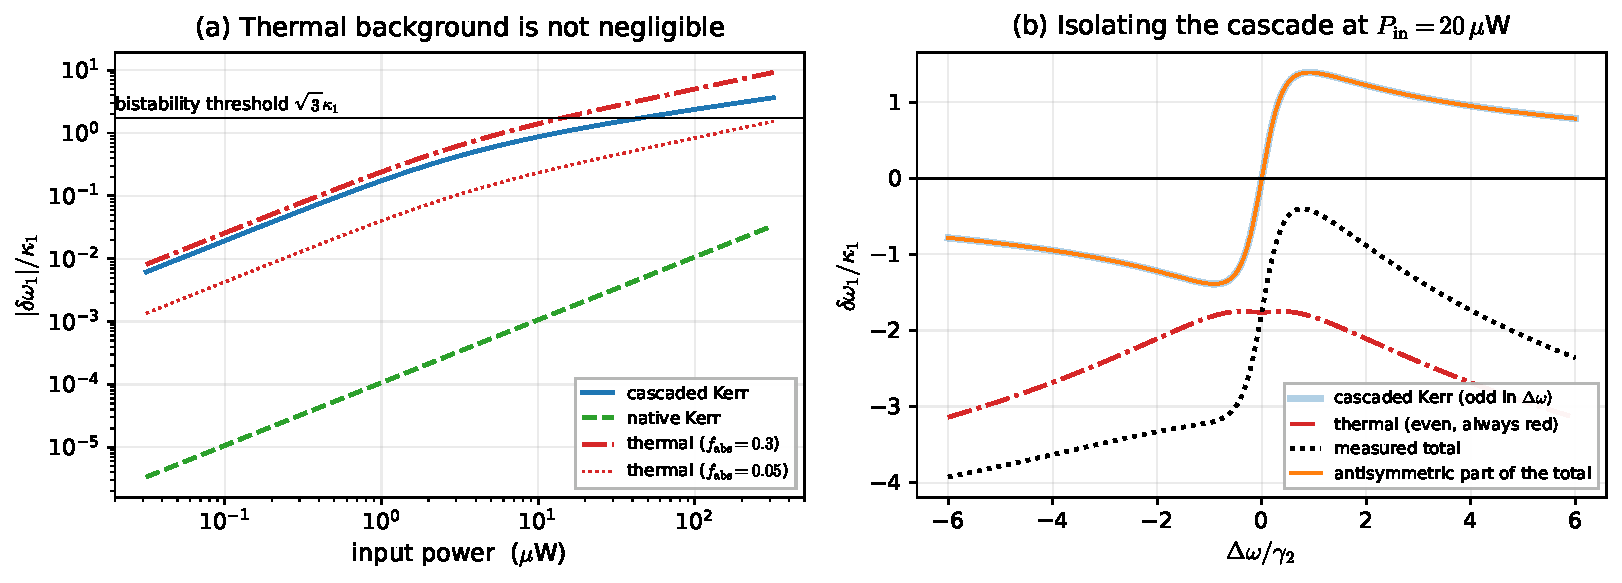
\includegraphics[width=\textwidth]{ring_thermal.pdf}
  \caption{(a) Resonance shift versus input power for the cascaded Kerr,
  the native Kerr and the thermal background at two absorbed fractions.
  The cascaded curve bends over because at $\delta_1=0$ the shift
  detunes the cavity from its own pump.  (b) At $20\,\mu$W the measured
  total (dotted) is thermally dominated, but its antisymmetric part
  (orange) reproduces the cascaded Kerr (thick blue) to $0.3\%$.}
  \label{fig:thermal}
\end{figure}

% =======================================================================
\section{Recommended experiment}\label{sec:experiment}

\begin{enumerate}[leftmargin=1.8em,itemsep=3pt]
\item \textbf{Device.}  A periodically poled LN microring, radius
  $30$--$70\,\mu$m, FM TM$_{00}$ at $1.55\,\mu$m critically coupled
  ($Q_1^{\text{load}}\simeq10^6$), SH TM$_{00}$ at $775$~nm left
  \emph{under-coupled} (the cascade wants the SH stored, not extracted).
  Add electrodes for $r_{33}$ tuning of $\Dom$.  A sister device with a
  deliberately out-coupled SH port is needed for step 2.
\item \textbf{Calibrate $g$.}  Measure $\etanorm$ in \%/W on double
  resonance and invert \eqref{eq:etaSHG}.  This fixes the absolute scale
  of every prediction in this note with no free parameters.  Measure
  $Q_1,Q_2$ (loaded and intrinsic) in the same run.
\item \textbf{Map $\Dom$.}  Temperature-tune to bring $\Dom$ through
  zero, identified by the maximum of SH power, and calibrate
  $d\Dom/dT$ ($\sim0.9$~GHz/K) and $d\Dom/dV$ against it.
\item \textbf{The sign-flip measurement.}  At fixed pump power
  ($10$--$50\,\mu$W), with the pump locked to the FM resonance
  ($\delta_1=0$, see Section~\ref{sec:competing}), dither $\Dom$
  electro-optically between $\pm2$--$4\,\gamma_2$ at $\gtrsim1$~MHz ---
  far above the thermal and photorefractive response, and well inside
  the cascade's own $2.6$~GHz bandwidth --- and lock-in
  detect the transmission, re-referencing $\Dom=0$ to the SH power
  maximum.  The in-phase component is
  $\propto\delta\omega_1^{\text{casc}}$ by \eqref{eq:antisym}.
  Sweep power to confirm linearity in $n$, and sweep $\Dom$ to trace the
  full dispersive lineshape of Figure~\ref{fig:signflip}(a).
\item \textbf{Bistability.}  Raise the power to $\sim50\,\mu$W at
  $\Dom\simeq+3.7\gamma_2$ and $\delta_1<0$; verify hysteresis, then
  reverse $\Dom$ and verify the hysteresis appears on the other side of
  the resonance.  This is the qualitative result no thermal mechanism
  can imitate.
\item \textbf{Control.}  Detune the SH far away ($|\Dom|\gg\gamma_2$) or
  temperature-tune off quasi-phase-matching, and repeat: the same device
  becomes the native-$\chithree$ reference.  \emph{The control experiment
  is the same chip.}
\end{enumerate}

The whole sequence needs microwatts, one tunable telecom laser, one
temperature controller, and the electrodes that thin-film LN already
has.  No amplifier, no pulsed source, and --- unlike the SH-only
metasurface samples --- no picosecond laser and no $Z$-scan.

% =======================================================================
\section{Numerical validation}\label{sec:validation}

Everything above was checked against direct integration of
\eqref{eq:cmt-a}--\eqref{eq:cmt-b}, non-dimensionalised
($\tau=\kappa_1t$, amplitudes in units of the linear-cavity amplitude)
and including the native Kerr term $+i\Unat|a|^2a$.  The transmission
lineshape from the full two-mode integration agrees with the closed-form
cubic \eqref{eq:cubic} to $4\times10^{-14}$ over the whole scan, which
is machine precision for this problem.  Additional checks, all reported
by \verb|ring_params.verify()|:

\begin{itemize}[leftmargin=1.6em,itemsep=2pt]
\item $\etanorm\leftrightarrow g$ inversion round trips to $<10^{-12}$,
  and \eqref{eq:etaSHG} matches the published Eq.~(4) of
  Ref.~\cite{Lu2020} analytically.
\item The linewidths recomputed from the quoted $Q$'s of
  Ref.~\cite{Lu2020} reproduce their $\kappa_{a,0}/2\pi=55.4$~MHz and
  $\kappa_{b,0}/2\pi=343.8$~MHz to $3\%$ (the residual is their quoted
  mode frequency of $199$~THz versus $2\pi c/1560$~nm).
\item The exact-versus-far-detuned ratio of $\Ucasc$ matches
  $[1+1/(4x^2)]^{-1}$ identically for $x=\Dom/\gamma_2$.
\item The bistability condition \eqref{eq:bist-cond} returns
  $|\delta_1|=\sqrt3\kappa_1$ at $\rho=0$, and the fixed-coefficient cusp
  formula agrees with a direct minimisation of the fold power over
  $\delta_1$ within that model to $0.1\%$.
\item The $4\times4$ Bogoliubov matrix of Section~\ref{sec:comb}
  reproduces its analytic $2\times2$ adiabatic reduction
  \eqref{eq:mi-local} to $9\times10^{-4}$ in the zero-walk-off limit,
  the residual being the finite-$\kappa_2$ correction to the
  elimination.  (An earlier comparison appeared to fail by a factor of
  two; the discrepancy was the FSR walk-off, which the reduction
  ignores and the $4\times4$ keeps.)
\item $n_2\leftrightarrow\chithree$ conversion round trips exactly.
\end{itemize}

\paragraph{What is \emph{not} verified.}  The three-wave couplings are
taken equal for every mode triplet; the thermal model is a lumped
single-time-constant estimate with an assumed absorption partition; no
photorefractive dynamics is modelled; and $g$ for Design~B is an
extrapolation (Section~\ref{sec:caveats}).

\begin{figure}[H]
  \centering
  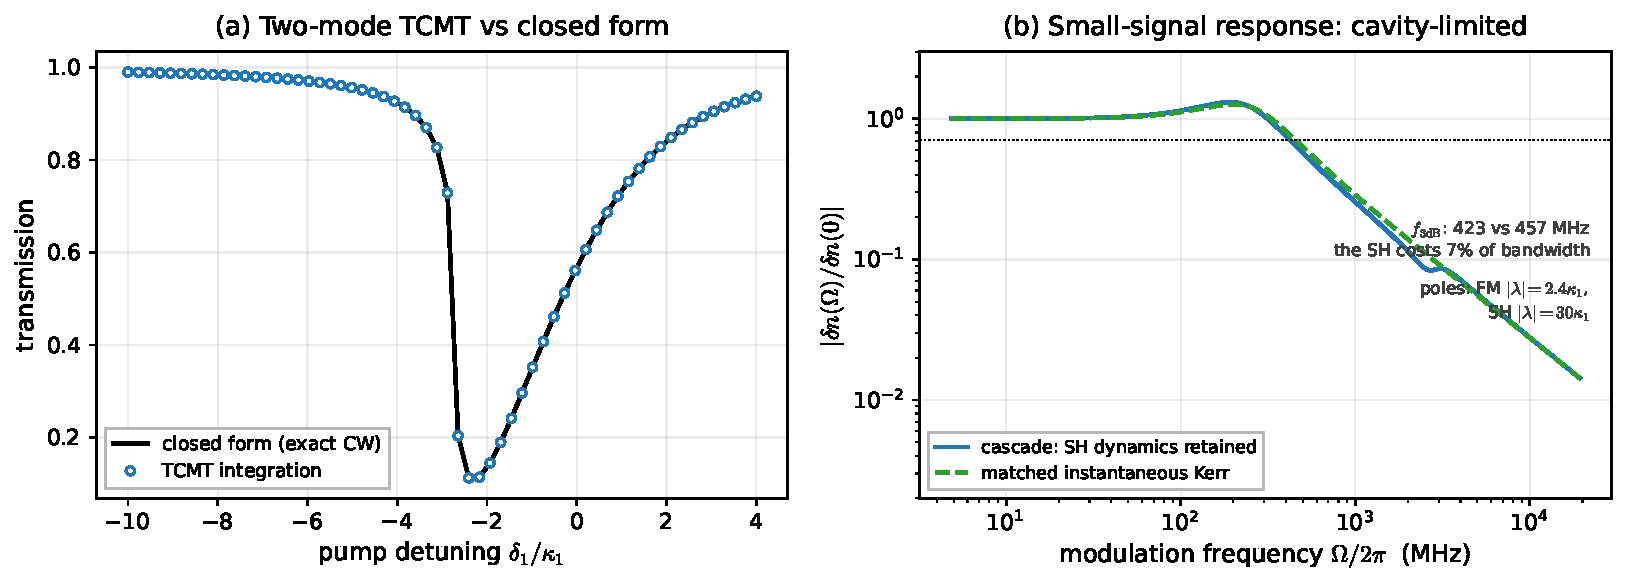
\includegraphics[width=\textwidth]{ring_validation.pdf}
  \caption{(a) Full two-mode TCMT integration against the closed-form
  steady state.  (b) Frequency response of the cascaded Kerr compared
  with the FM cavity: the cascade rolls off at $\Dom/2\pi=2.6$~GHz, the
  matched instantaneous-Kerr reference: the SH's finite response time
  costs $7\%$ of modulation bandwidth, so the resonator is the
  bottleneck (Rule~1).}
  \label{fig:validation}
\end{figure}

% =======================================================================
\section{Comparison across platforms and architectures}\label{sec:compare}

\begin{table}[H]
\centering
\small
\begin{tabular}{p{3.9cm}ccc}
\toprule
 & metasurface (note \S10) & SH-only samples & \textbf{PPLN microring} \\
\midrule
$Q_2$                          & $4\times10^3$ & $0.9$--$5.6\times10^3$ & $3$--$6\times10^5$\\
overlap mechanism              & meta-atom & meta-atom & QPM over $2\pi R$\\
$R$ at $\Dom=2\gamma_2$        & $\sim12$ & $0.4$--$2.5$ & $\bm{1.8\times10^3}$\\
absolute scale known?          & prefactor $\times4$ & $+\,C_{\text{bridge}}$ & \textbf{yes, from} $\etanorm$\\[1pt]
bandwidth bottleneck           & SH ($\gamma_2<\gamma_1$) & SH & \textbf{FM cavity}\\
CW Kerr device?                & marginal & no ($\mu$rad) & \textbf{yes, at $\mu$W}\\
sign flip observable?          & yes & yes (ps $Z$-scan) & \textbf{yes, CW + lock-in}\\
principal risk                 & disorder & overlap & thermal, photorefr.\\
\bottomrule
\end{tabular}
\caption{The microring platform against the two metasurface platforms
studied earlier in this project.}
\label{tab:platforms}
\end{table}

Against the \emph{native}-$\chithree$ architecture on the same ring, the
cascade wins on every intensity-dependent observable by two to three
orders of magnitude in threshold power, wins outright on sign
tunability, very nearly breaks even on speed (the SH costs $7\%$ of
modulation bandwidth), and loses on three counts: it introduces a nonlinear loss channel that TPA-free LN
does not otherwise have; it requires the doubly-resonant condition to be
held to a fraction of $\gamma_2$; and it is mode-selective across a comb
where the native Kerr is uniform.

% =======================================================================
\section{Caveats and what would change the answer}\label{sec:caveats}

In rough order of how much they could move the headline:

\begin{enumerate}[leftmargin=1.8em,itemsep=3pt]
\item \textbf{$Q_2$ at $775$~nm is assumed, not measured on this
  process} ($3\times10^5$ loaded, $6\times10^5$ intrinsic, taken from
  Ref.~\cite{Lu2020}).  Loaded values of this order near $780$--$800$~nm
  are experimentally plausible and have precedent, but we do not claim
  they are routine, and the intrinsic ceiling in high-quality thin-film
  LN is higher than the value used here~\cite{Zhang2017}.  Since
  $R\propto Q_2$ this is the single largest lever: an order of magnitude
  down in $Q_2$ is an order of magnitude down in $R$, though even
  $Q_2=10^4$ leaves $R\simeq61$.  The floor is
  $Q_2^{\text{cross}}=164$, below which the cascade loses to the native
  Kerr.
\item \textbf{Periodic poling must be available.}  Without it
  $R$ drops from $\sim1.8\times10^3$ to $\sim13$
  (Table~\ref{tab:summary}), thresholds rise into the milliwatt range
  where thermal effects dominate, and the experiment reverts to being as
  hard as the metasurface version.  Everything in this note hinges on
  this one fabrication capability.
\item \textbf{$g$ for Design~B is extrapolated}, scaled as
  $\Veff^{-1/2}$ from the $70\,\mu$m device of Ref.~\cite{Lu2020} at
  fixed $\Aeff=1\,\mu$m$^2$.  Poling fidelity and duty-cycle error
  degrade with radius, so this is optimistic at the $\sim30\%$ level in
  $g$, i.e.\ up to $\sim2\times$ in $R$.  Step~2 of
  Section~\ref{sec:experiment} measures it directly and removes the
  issue.
\item \textbf{The native LN Kerr is quoted at the pessimistic end.}  We
  use $n_2=1.8\times10^{-19}$~m$^2$/W; reported values span
  $0.9$--$1.8\times10^{-19}$, and the smaller value would \emph{raise}
  $R$ by up to $2\times$.  The choice is deliberately conservative.
\item \textbf{The thermal model is lumped and order-of-magnitude}
  ($R_{\text{th}}=3\times10^4$~K/W, absorbed fraction $0.05$--$0.3$ of
  the intrinsic loss, single time constant).  It is used only to
  establish that the thermal background is comparable to or larger than
  the cascaded Kerr, which is robust across that whole parameter range;
  none of the cascade physics depends on it.
\item \textbf{Photorefractive drift is a real and unquantified risk} at
  exactly the $\gtrsim10\,\mu$W powers of interest~\cite{Lu2020}.  It
  acts on $\Dom$ itself, so it corrupts the control variable rather than
  just the readout.  Cladding removal~\cite{Xu2021}, elevated
  temperature and MgO doping are the known mitigations; none is free.
\item \textbf{Comb applications need more than the two-mode model.}
  Section~\ref{sec:comb} establishes the parametric threshold
  rigorously, but the FM/SH free-spectral-range walk-off makes the
  cascade mode-selective, so a genuine comb calculation requires the
  multimode $\chitwo$ model, not the effective Kerr used here.
\item \textbf{The $\eta_{\text{geom}}=0.93$ implied by the metasurface
  note's formula sits at its physical ceiling}
  (Section~\ref{sec:R}), which points either to the larger
  $\beta$-prefactor branch or to an overestimated $\Aeff$; as
  Section~\ref{sec:anchor} says, a scalar estimate cannot separate the
  two.  It does not affect any microring number in this note, all of
  which are anchored on the measured $g$, but it does need resolving
  before the two notes are quoted side by side.
\item \textbf{Equal three-wave couplings are assumed} across every mode
  triplet in the multimode calculation, and for the XPM factor of two.
  In a real ring $g_{12c}\neq g_{11b}$ because the frequencies, transverse
  profiles, tensor projections and QPM overlaps all differ.
\end{enumerate}

% =======================================================================
\section{Summary and recommendation}\label{sec:summary}

\begin{enumerate}[leftmargin=1.8em,itemsep=3pt]
\item A doubly-resonant PPLN microring on the quoted platform
  ($Q_1^{\text{load}}\sim10^6$, $Q_1^{\text{int}}\sim2\times10^6$) with
  the demonstrated coupling $g/2\pi\simeq1.2$--$1.4$~MHz yields
  $R\simeq1.8\times10^3$ at $\Dom=2\gamma_2$, i.e.\
  $n_2^{\text{eff}}\simeq-3.3\times10^{-16}$~m$^2$/W.  This is three
  orders of magnitude better than anything the metasurface route
  delivered, and the reason is $Q_2$ and quasi-phase matching, not luck.
\item \textbf{Periodic poling is the enabling step.}  Without it,
  $R\simeq13$ --- the same order as the metasurface --- and the
  crossover $Q_2$ rises from $164$ to $2.4\times10^4$.
\item The absolute scale is measurable, not modelled: $\etanorm$ in
  \%/W fixes $g$ through \eqref{eq:etaSHG}.  This removes the
  $C_{\text{bridge}}$ unknown that limited the SH-only sample analysis,
  and incidentally provides the first external evidence on the main
  note's $\beta$-prefactor ambiguity, favouring the larger branch.
\item Design rules: bistability and single-pair parametric gain both
  need the \emph{pump-frame} ratio $\rho=\kappa_2/|\Delta_{\text{eff}}|$
  to satisfy $\rho<1/\sqrt3$ --- a condition on $\Delta_{\text{eff}}=\Dom-2\delta_1$,
  which the experimenter controls, not a fabrication requirement on
  $\Dom$; the Kerr description needs
  $\Omega_{\text{env}}\ll\sqrt{\kappa_2^2+\delta_2^2}=27\kappa_1$ here;
  and the shift stays linear up to $|\delta\omega_1|\sim\Dom$, which is
  $8Q_1/Q_2$ linewidths and therefore ample.  The recommended cold-cavity
  operating point is $\Dom\simeq3\gamma_2$, not $2\gamma_2$.
\item Thresholds: bistability at $32$--$37\,\mu$W (native $14$~mW),
  parametric oscillation at $8.4\,\mu$W from a multimode Bogoliubov
  calculation (native $9.4$~mW), switching at $8.4$~fJ intracavity,
  $13\,\mu$W of CW drive (native $15.4$~pJ, $19$~mW).
\item The cascade is a classical instrument, not a quantum one.  Its
  dispersive anharmonicity is $\sim(g/\kappa_1)(g/\kappa_2)$; blockade
  needs resonant operation instead.
\item The binding constraints are thermal and photorefractive shifts,
  within a factor of two of the cascaded Kerr at these powers.  To
  leading order both are even in $\Dom$ where the cascade is odd, and
  LN's own Pockels effect tunes $\Dom$ by $2.4\gamma_2$ per V/$\mu$m and
  far faster than either background responds.  Photorefraction is not
  guaranteed to be exactly even, so any residual odd background must be
  bounded experimentally.  The recommended first experiment is therefore an
  electro-optically dithered, antisymmetric-in-$\Dom$ lock-in
  measurement of the FM resonance shift at $10$--$50\,\mu$W, with the
  same chip serving as its own native-$\chithree$ control.
\end{enumerate}

\paragraph{Recommendation.}  The microring platform is well suited to
this physics --- substantially better than the metasurface platform this
project started from --- and the decisive experiment is a CW,
microwatt-level, room-temperature measurement on a single chip.  The
two open questions worth settling before committing are the SH quality
factor actually achievable at $775$~nm on this process, and whether
periodic poling is available; the second is worth far more than the
first.

% =======================================================================
\appendix
\section{Reproducing the numbers}\label{app:code}

All numbers and figures come from two modules in
\texttt{cascaded\_chi3/}:

\begin{itemize}[leftmargin=1.6em,itemsep=2pt]
\item \texttt{ring\_params.py} --- \texttt{RingParams} dataclass, the
  design points of Table~\ref{tab:designs}, the closed forms
  \eqref{eq:Ucasc}--\eqref{eq:R}, the $\etanorm\leftrightarrow g$
  inversion \eqref{eq:etaSHG}, the bistability algebra
  \eqref{eq:bist-cond}, and the thermal/electro-optic tuning of $\Dom$.
  Running it prints the eight-part verification report of
  Section~\ref{sec:validation}.
\item \texttt{ring\_effects.py} --- the exact CW cubic, the
  non-dimensionalised two-mode TCMT integrator, the $4\times4$
  linear-stability analysis, and the figure set in
  \texttt{cascaded\_chi3/figures/ring/}.
\end{itemize}

\noindent
Both run standalone: \verb|conda run -n ml_base python ring_params.py|,
then \verb|ring_effects.py|.  They are deliberately not wired into
\texttt{run\_all.py}, which builds the main-note figures only.

% =======================================================================
\begin{thebibliography}{99}

\bibitem{Lu2020}
J.~Lu, M.~Li, C.-L.~Zou, A.~Al~Sayem, and H.~X.~Tang,
``Toward 1\% single-photon anharmonicity with periodically poled lithium
niobate microring resonators,''
\emph{Optica} \textbf{7}, 1654--1659 (2020); arXiv:2007.07411.

\bibitem{Lu2019}
J.~Lu, J.~B.~Surya, X.~Liu, A.~W.~Bruch, Z.~Gong, Y.~Xu, and H.~X.~Tang,
``Periodically poled thin-film lithium niobate microring resonators with
a second-harmonic generation efficiency of 250,000\%/W,''
\emph{Optica} \textbf{6}, 1455--1460 (2019).

\bibitem{Zhang2017}
M.~Zhang, C.~Wang, R.~Cheng, A.~Shams-Ansari, and M.~Lon\v{c}ar,
``Monolithic ultra-high-$Q$ lithium niobate microring resonator,''
\emph{Optica} \textbf{4}, 1536--1537 (2017).

\bibitem{Xu2021}
Y.~Xu, M.~Shen, J.~Lu, J.~B.~Surya, A.~Al~Sayem, and H.~X.~Tang,
``Mitigating photorefractive effect in thin-film lithium niobate
microring resonators,''
\emph{Opt.\ Express} \textbf{29}, 5497--5504 (2021).

\bibitem{QuadraticComb2024}
C.~Tang, M.~Nie, J.-Y.~Chen, Z.~Ma, Z.~Li, Y.~Xie, Y.~M.~Sua,
S.-W.~Huang, and Y.-P.~Huang,
``Broadband frequency comb generation through cascaded quadratic
nonlinearity in thin-film lithium niobate microresonators,''
\emph{Opt.\ Lett.} \textbf{49}, 2449--2452 (2024);
doi:10.1364/OL.518722.

\bibitem{DeSalvo1992}
R.~DeSalvo, D.~J.~Hagan, M.~Sheik-Bahae, G.~Stegeman, E.~W.~Van~Stryland,
and H.~Vanherzeele,
``Self-focusing and self-defocusing by cascaded second-order effects in
KTP,''
\emph{Opt.\ Lett.} \textbf{17}, 28--30 (1992).

\bibitem{Stegeman1996}
G.~I.~Stegeman, D.~J.~Hagan, and L.~Torner,
``$\chi^{(2)}$ cascading phenomena and their applications to all-optical
signal processing, mode-locking, pulse compression and solitons,''
\emph{Opt.\ Quantum Electron.} \textbf{28}, 1691--1740 (1996).

\bibitem{Khurgin1997}
J.~B.~Khurgin, A.~Obeidat, S.~J.~Lee, and Y.~J.~Ding,
``Cascaded optical nonlinearities: microscopic understanding as a
collective effect,''
\emph{J.\ Opt.\ Soc.\ Am.\ B} \textbf{14}, 1977--1983 (1997).

\bibitem{Kippenberg2018}
T.~J.~Kippenberg, A.~L.~Gaeta, M.~Lipson, and M.~L.~Gorodetsky,
``Dissipative Kerr solitons in optical microresonators,''
\emph{Science} \textbf{361}, eaan8083 (2018).

\bibitem{Boyd}
R.~W.~Boyd, \emph{Nonlinear Optics}, 4th ed. (Academic Press, 2020).

\end{thebibliography}

\end{document}
